%!TEX root=./LIVRO.tex
\setcounter{chapter}{0}
\chapter[Simulado 1]{Simulado}

\num{1} Observe o cartaz abaixo para responder à questão.


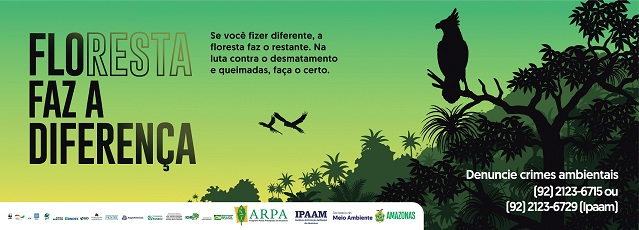
\includegraphics[width=5.90551in,height=2.125in]{./imgSAEB_7_POR/media/image16.png}

\fonte{Secretaria do Meio Ambiente do Estado do Amazonas. Campanha Floresta faz a diferença. 
Disponível em: https://meioambiente.am.gov.br/campanha-floresta-faz-a-diferenca/.
Acesso em: 22 mai. 23}

\noindent Acima, pode-se observar um cartaz de conscientização sobre o desmatamento da
Amazônia. O uso e repetição de determinadas palavras e imagens tem como
finalidade sensibilizar os leitores para o problema do desmatamento.
Sobre o uso da palavra ``floresta'', no cartaz, assinale a alternativa
correta.

\begin{escolha}

  \item Destacada à esquerda em letras grandes, uma parte da palavra ``floresta'' compõe um jogo com 
  palavras do texto no centro do cartaz.   

  \item A parte destacada da palavra ``floresta'', à esquerda, remete aos malefícios das queimadas e desmatamento que o cartaz pretende combater. 

  \item O destaque da palavra ``floresta'' não dialoga com ``diferença'' e ``diferente'', que se articulam para convidar a uma mudança de atitude.

  \item O uso da palavra ``floresta'', em destaque, à esquerda, dialoga com as imagens à direita sem remeter ao texto central do cartaz da campanha. 

\end{escolha}

\num{2} Leia o texto abaixo para responder à questão. 

\begin{myquote}
\textbf{Fumaça de queimadas chega a São Paulo}

\textit{Segundo especialistas, a grossa nuvem de fumaça começou com incêndios nos estados das regiões
Norte e Centro-Oeste.}

No dia 9 de sexta-feira, moradores da cidade de São Paulo relataram sentir
um forte cheiro de fumaça. Esse fenômeno estava relacionado com uma nuvem
de fumaça proveniente de queimadas que haviam ocorrido nos estados do
Amazonas, Acre e Mato Grosso. Especialistas já haviam alertado sobre a
propagação dessa nuvem sobre o Brasil, prevendo que atingiria também grande
parte do Centro-Oeste, do Paraná e até mesmo parte do estado de São Paulo.

Diante dessa situação, a Companhia Ambiental do Estado de São Paulo (CETESB)
iniciou uma investigação para analisar as condições do ar na região
metropolitana de São Paulo. A divisão de Qualidade do Ar da agência está
detalhando os dados provenientes das estações de monitoramento e se
comprometeu a fornecer informações mais consolidadas assim que concluírem sua
apuração.

\fonte{Fonte de pesquisa: Ingrid Oliveira e Carolina Figueiredo. Fumaça de queimadas do Amazonas chega a São Paulo; 
moradores relatam ``cheiro forte''. Disponível em:
https://www.cnnbrasil.com.br/nacional/fumaca-de-queimadas-do-amazonas-chega-a-sao-paulo-moradores-relatam-cheiro-forte/.
Acesso em: 22 mai. 2023.}

\end{myquote}

Assinale a alternativa que contém a parte da notícia denominada linha fina.

\begin{escolha}

\item ``moradores da cidade de São Paulo relataram sentir um forte cheiro de fumaça''.

\item ``Especialistas já haviam alertado sobre a propagação dessa nuvem sobre o Brasil''.

\item ``a Companhia Ambiental do Estado de São Paulo (CETESB)
iniciou uma investigação para analisar as condições do ar''.

\item ``Segundo especialistas, a grossa nuvem de fumaça começou com incêndios nos estados das regiões
Norte e Centro-Oeste''.

\end{escolha}

\num{3} Leia o texto abaixo para responder à questão.

\begin{myquote}
Uma parceria entre a Universidade Federal do Rio de Janeiro e a
Universidade Federal do Estado do Rio de Janeiro (Unirio) vem estudando
o vírus-T linfotrópico humano do tipo 1, o HTLV-1, retrovírus da mesma
família do HIV, associado a casos de leucemia e doenças
neurodegenerativas. A pesquisa recebeu investimento da Organização
Pan-Americana de Saúde (Opas/OMS) junto com outros estudos
latino-americanos e caribenhos que investigam doenças negligenciadas.
Embora descrito, na década de 1980, como um vírus associado ao câncer, o
HTLV ainda é pouco estudado e bastante desconhecido do público em geral.

\fonte{Carol Correia e Luana Reis.Conexão UFRJ. 
Pesquisa investiga vírus que pode levar à leucemia e neurodegeneração.
Disponível em: https://conexao.ufrj.br/2023/04/pesquisa-investiga-virus-negligenciado-que-pode-levar-a-doencas-neurodegenerativas-e-leucemia/.
Acesso em: 22 mai. 2023.}

\end{myquote}

O texto acima pertence ao gênero de divulgação científica, pois:

\begin{escolha}
  
  \item traz informações técnicas e de difícil compreensão.
  
  \item é escrito de maneira formal e dirigido a cientistas e estudiosos.
  
  \item traz informações sobre fatos do cotidiano.
  
  \item traz informações científicas em linguagem clara e acessível ao público.

\end{escolha}

\pagebreak

\num{4} Leia o texto abaixo para responder à questão.

\begin{myquote}

Ilma. Sra. Diretora da Escola Estadual Ulysses Guimarães:

Mariana Amaral Santos, aluna regularmente matriculada no sétimo ano do
Ensino Fundamental desta escola, vem respeitosamente solicitar à V.S.\textsuperscript{a} a
expedição dos documentos necessários à sua transferência para outro
estabelecimento de ensino.

Nestes termos, pede deferimento.

Curitiba, 24 de setembro de 2022.

\fonte{Texto adaptado para este material.}

\end{myquote}

O texto acima é um modelo de requerimento, pois tem como objetivo:

\begin{escolha} 

\item convencer o destinatário a realizar uma ação importante.

\item solicitar formalmente ao destinatário a realização de uma ação.

\item mudar o comportamento do destinatário a partir da realização de ações.

\item informar formalmente o destinatário acerca da solicitação de ações.

\end{escolha}

\num{5} Leia o texto abaixo para responder à questão.

\begin{myquote}

\textbf{ATO I}

\textbf{Cena I}

\textit{Veneza. Uma rua. Entram Antônio, Salarino e Salânio.}

ANTÔNIO -- Não sei, realmente, porque estou tão triste. Isso me enfara; e
a vós também, dissestes. Mas como começou essa tristeza, de que modo a
adquiri, como me veio, onde nasceu, de que matéria é feita, ainda estou
por saber. E de tal modo obtuso ela me deixa, que mui dificilmente me
conheço.

SALARINO -- Vosso espírito voga em pleno oceano, onde vossos galeões de
altivas velas -- como burgueses ricos e senhores das ondas, ou qual vista
aparatosa distendida no mar -- olham por cima da multidão de humildes
traficantes que os saúdam, modestos, inclinando-se, quando perpassam com
tecidas asas.

\fonte{William Shakespeare. O Mercador de Venza. 
Disponível em: http://www.dominiopublico.gov.br/download/texto/cv000094.pdf.
Acesso em: 22 mai. 2023.}

\end{myquote}

O trecho acima apresenta certas características, como discurso direto,
indicações de falas de personagens e rubricas, que são características 

\begin{escolha}

  \item das peças de teatro, textos escritos para encenação.

  \item dos poemas, compostos por versos e estrofes.

  \item dos contos, narrações curtas e de alto impacto.

  \item dos romances, narrativa longas e complexas.

\end{escolha}

\num{6} Leia o texto abaixo para responder à questão. 

\begin{myquote}

Os sites de fofoca são frequentemente alvo de críticas, mas eu sou
um firme defensor de sua existência. É um prazer de acompanhar a vida de celebridades
e figuras públicas, muitas vezes revelando verdades incômodas que a mídia tradicional 
ignora. Além disso, eles oferecem uma fonte interminável de diversão para milhões de
pessoas, servindo como uma fuga bem-vinda da monotonia da vida cotidiana. A
fofoca é sinal de uma cultura vibrante.

\fonte{Texto formulado para este material, escrito a partir de comentários 
em sites de fofoca e páginas de celebridades nas redes sociais.}

\end{myquote}

O texto acima contém muitas opiniões e poucos fatos. Há um fato
expresso no texto em:

\begin{escolha}

  \item ``Os sites de fofoca são frequentemente alvo de críticas''.
  
  \item ``É um prazer de acompanhar a vida de celebridades''.
  
  \item ``eles oferecem uma fonte interminável de diversão''.
  
  \item ``A fofoca é sinal de uma cultura vibrante''.

\end{escolha}

\num{7} Leia o texto abaixo para responder à questão.

%Alterei a questão. Rogério, 24/5/23, 10h13
%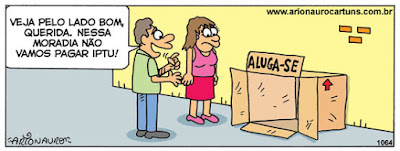
\includegraphics[width=4.16667in,height=1.57292in]{./imgSAEB_7_POR/media/image17.png}
%\fonte{http://www.arionaurocartuns.com.br/search?q=moradia}{\uline{http://www.arionaurocartuns.com.br/search?q=moradia}}.
%Acesso em 20 de Abr de 2023.

\begin{myquote}

É inútil descrever o quarto de um estudante: aí nada se
encontra de novo. Ao muito acharão uma estante, onde ele guarda
os seus livros, um cabide, onde pendura a casaca, o moringue, o
castiçal, a cama, uma até duas canastras de roupa, o chapéu, a
bengala e a bacia, a mesa, onde escreve e que só apresenta de
recomendável a gaveta cheia de papéis, de cartas de família, de
flores e fitinhas misteriosas: é pouco mais ou menos assim o
quarto de Augusto.

Agora ele está só. Às sete horas, desse quarto saíram três
amigos: Filipe, Leopoldo e Fabrício. Trataram da viagem no dia 
seguinte e retiraram-se descontentes.

\fonte{Joaquim Manuel de Macedo. \textit{A moreninha}.} 

\end{myquote}

% \fonte{Joaquim Manuel de Macedo. A moreninha. 
% Disponível em: http://objdigital.bn.br/Acervo_Digital/Livros_eletronicos/a_moreninha.pdf.
% Acesso em: 24 mai. 2023.}

Assinale a alternativa correta quanto aos trechos do texto.

\begin{escolha}
    
    \item ``\textbf{aí} nada se encontra de novo'': o termo destacado se refere a ``um estudante''.
    
    \item ``onde escreve'': o sentido da frase equivale a ``onde eles escrevem''.  
    
    \item ``o quarto de Augusto'': Augusto é o estudante cujo quarto é citado no início do parágrafo.  
    
    \item ``Agora \textbf{ele} está só'': o termo destacado refere-se a ``o quarto de Augusto''.   

\end{escolha}

\pagebreak

\num{8} Leia o texto abaixo para responder à questão. 

%Tirei a imangem abaixo e alterei a questão (Rogério, 24/5/23, 9h52)
%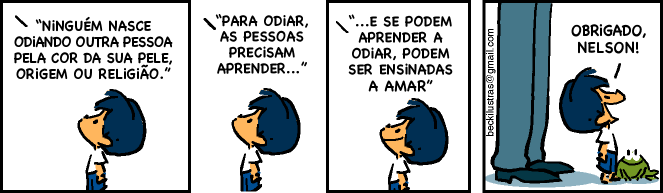
\includegraphics[width=5.90551in,height=1.72222in]{./imgSAEB_7_POR/media/image18.png}
%\fonte{https://tirasarmandinho.tumblr.com/search/amor}{\uline{https://tirasarmandinho.tumblr.com/search/amor}}.
%Acesso em 21 de Abr.

\begin{myquote}

--- Não diga isso, Camilo. Se você soubesse como eu tenho andado, por sua
causa. Você sabe; já lhe disse. Não ria de mim, não ria \ldots{}

Camilo pegou-lhe nas mãos, e olhou para ela sério e fixo. Jurou que lhe
queria muito, que os seus sustos pareciam de criança; em todo o caso,
quando tivesse algum receio, a melhor cartomante era ele mesmo. Depois,
repreendeu-a; disse-lhe que era imprudente andar por essas casas.

\end{myquote}

% \fonte{Machado de Assis. A cartomante. Disponível em: 
% http://www.dominiopublico.gov.br/download/texto/bv000257.pdf.
% Acesso em: 23 mai. 2023.}
\fonte{Machado de Assis. \textit{A cartomante}.}

O diálogo acima pertence ao conto ``A cartomante'', de Machado de Assis.
No primeiro parágrafo, Rita lamenta ao amante Camilo o que vem 
sofrendo por ele. Assinale a alternativa correta quanto aos 
referentes dos pronomes destacados.  

\begin{escolha}

  \item ``\textbf{Você} sabe; já \textbf{lhe} disse'': os pronomes se referem a Rita.
  
  \item ``Camilo pegou-\textbf{lhe} nas mãos'': o pronome se refere às mãos de Camilo.
  
  \item ``Jurou que \textbf{lhe} queria muito'': o pronome se refere a Camilo.
  
  \item ``disse-\textbf{lhe} que era imprudente'': o pronome se refere a Rita.

\end{escolha}

\num{9} Leia o texto abaixo para responder à questão.

\begin{myquote}

Para nós, indígenas, uma montanha não é apenas uma formação geológica, mas sim
uma pessoa sagrada. Ela é parte essencial da nossa vida e cultura, e a
respeitamos como tal. A montanha não é vista como um mero recurso econômico,
mas como um ser vivo que desempenha um papel vital em nossa história e
espiritualidade. 

\fonte{Texto fomulado para este material. Fonte de pesquisa: Ailton Krenak. \textit{Ideias para adiar o fim do mundo}. 2ª Ed. São Paulo:
Companhia da Letras, 2020.}

\end{myquote}

No texto acima, o autor

\begin{escolha}

  \item contou narrativas tradicionais da cultura indígena.

  \item comparou pontos de vista de indígenas e não indígenas.

  \item apresentou a língua falada pelo seu povo indígena.

  \item conciliou a cosmovisão de indígenas e não indígenas.

\end{escolha}

\num{10} Leia o texto abaixo para responder à questão.

\begin{myquote}

\textbf{Limpeza adequada evita crise alérgica e problemas
respiratórios}

Desde a infância, Maria Fulânima da Silva, aposentada de 53 anos, sofre com alergias, e
seus problemas respiratórios pioraram consideravelmente após o diagnóstico de
Lúpus, devido à sua baixa imunidade associada à doença. \textbf{Por causa disso}, ela
teve que intensificar os cuidados na organização de sua casa. Especialistas
advertem que pessoas alérgicas devem evitar acumular certos objetos,
especialmente no quarto, e, em vez de usar vassoura para a limpeza do chão,
recomendam o uso de um pano úmido. Eles também compartilham dicas sobre como
manter a residência limpa sem comprometer a saúde.

\fonte{Fonte de pesquisa: Jornal da Paraíba. Disponível em: https://jornaldaparaiba.com.br/bichos/faxina-correta-da-casa-evita-crise-alergica-e-possiveis-problemas-respiratorios/.
Acesso em: 2 out. 2023.}

\end{myquote}

No texto acima, a expressão destacada se refere:

\begin{escolha}
  
  \item à limpeza redobrada do ambiente.
  
  \item ao agravamento dos problemas respiratórios.
  
  \item à orientação médica sobre os cuidados com as crianças.
  
  \item à idade da paciente que precisa de cuidados.

\end{escolha}

\num{11} Leia o texto a seguir para responder à questão.

\begin{myquote}

O uso excessivo de celulares ocupa tempo precioso. As notificações constantes
e a busca por conteúdo online podem nos afastar do mundo real,
prejudicando nossa capacidade de conexão genuína com as pessoas ao nosso
redor. Além disso, o vício em smartphones é uma âncora que nos impede de
explorar as experiências e oportunidades que a vida tem a oferecer. Isso pode
levar a problemas de saúde mental, como ansiedade e depressão, bem como a uma
diminuição da produtividade e da qualidade de vida. É fundamental equilibrar
nosso uso de celulares para não nos perdermos no mundo virtual e manter um
vínculo sólido com a realidade que nos cerca.

\fonte{Texto formulado para este material.}

\end{myquote}

% \textbf{Sedentários e grudados a uma tela. O
% que mostra o maior estudo mundial sobre atividade física de
% jovens}

% Os especialistas já há algum tempo vêm alertando que os jovens não fazem todo o exercício físico que deveriam. Agora temos a confirmação: 80\% dos adolescentes (11 a 17 anos) em todo o mundo não fazem a atividade diária mínima para estarem saudáveis. E os especialistas não falam só de praticar esportes, e sim de ações básicas como caminhar até a escola ou jogar bola com os amigos no parque. Os padrões da Organização Mundial da Saúde (OMS) falam de uma hora diária de movimento. Estes dados ganham agora uma nova relevância se levarmos em conta a epidemia de obesidade que alcançou praticamente todos os países do mundo.

% \fonte{Patrícia Peiró. El País Brasil. Disponível em: https://brasil.elpais.com/brasil/2019/11/18/actualidad/1574086350_697117.html.
% Acesso em: 23 mai. 2023.}
%\fonte{Patrícia Peiró. El País Brasil.}

A frase que contém uso de figura de linguagem é:

\begin{escolha}
    
    \item ``O uso excessivo de celulares ocupa tempo precioso''.
    
    \item ``As notificações constantes e a busca por conteúdo online podem nos afastar do mundo real''.
    
    \item ``o vício em smartphones é uma âncora que nos impede de explorar as experiências''.
    
    \item ``pode levar a problemas de saúde mental, como ansiedade e depressão''.

\end{escolha}

\num{12} Leia o texto abaixo para responder á questão.

\begin{myquote}

Lisboa, situada em uma área geologicamente ativa, está sujeita à possibilidade
de ocorrer um grande terremoto nos próximos anos. A cidade já experimentou
eventos sísmicos significativos ao longo de sua história, como o terremoto de
1755, que causou devastação considerável. A região é parte da Zona de
Convergência da Eurásia e da África, onde as placas tectônicas se encontram,
aumentando o risco de atividade sísmica. Embora seja impossível prever com
precisão quando um novo evento pode ocorrer, as autoridades em Lisboa têm
tomado medidas de preparação e conscientização para minimizar os potenciais
danos e garantir a segurança da população.

\fonte{Texto formulado para este material.}

\end{myquote}

% \fonte{Oriol Güell. El País Brasil. Agência de saúde pública da UE avisa
% que a ômicron se propaga pelo continente mais rápido do que é detectada.
% Disponível em: https://brasil.elpais.com/internacional/2021-12-13/agencia-de-saude-publica-da-ue-avisa-que-a-omicron-se-propaga-pelo-continente-mais-rapido-do-que-e-detectada.html.
% Acesso em: 23 mai. 2023.}
%\fonte{Oriol Güell. El País Brasil.}

A expressão ``um novo evento'' se refere a:

\begin{escolha}
  
  \item ``um grande terremoto nos próximos anos''.
  
  \item ``o terremoto de 1755''.
  
  \item ``risco de atividade sísmica''.
  
  \item ``potenciais danos''.

\end{escolha}

\pagebreak

\num{13} Leia o texto abaixo para responder à questão. 

\begin{myquote}

A defesa da prática da leitura nas escolas brasileiras é respaldada por
estatísticas que evidenciam seus benefícios. De acordo com o último
levantamento do Instituto Pró-Livro, realizado em 2019, apenas 52\% da
população brasileira afirma ter lido ao menos um livro nos últimos três meses.
Esse número ressalta a necessidade de incentivar a leitura desde cedo, nas
escolas, como uma ferramenta poderosa para o desenvolvimento cognitivo e
educacional dos alunos. Além disso, dados do Programa Internacional de
Avaliação de Estudantes (PISA) demonstram que estudantes que têm o hábito de
leitura apresentam desempenho superior em todas as disciplinas, incluindo
matemática e ciências. Promover a leitura nas escolas não apenas
contribui para o crescimento intelectual dos estudantes, mas também pode ser
um meio eficaz de melhorar a qualidade da educação no Brasil.

\end{myquote}

% \fonte{Ana Cássia Maturano. G1. Opinião: como fazer de seu filho um leitor. 
% Disponível em: https://g1.globo.com/Noticias/Vestibular/0,,MUL723077-5604,00-OPINIAO+COMO+FAZER+DE+SEU+FILHO+UM+LEITOR.html.
% Acesso em: 22 mai. 2023.}
%\fonte{Ana Cássia Maturano. G1. Opinião: como fazer de seu filho um leitor.}

Para defender a prática da leitura nas escolas brasileiras, o autor do texto 
acima usou 

\begin{escolha}

    \item opiniões de especialistas, alunos e professores.

    \item exemplos de sucesso em escolas brasileiras. 

    \item dados estatísticos de fontes confiáveis.

    \item afirmações genéricas que não podem ser refutadas. 

\end{escolha}

\pagebreak

\num{14} Observe a imagem a seguir para responder à questão.

\begin{figure}[H]
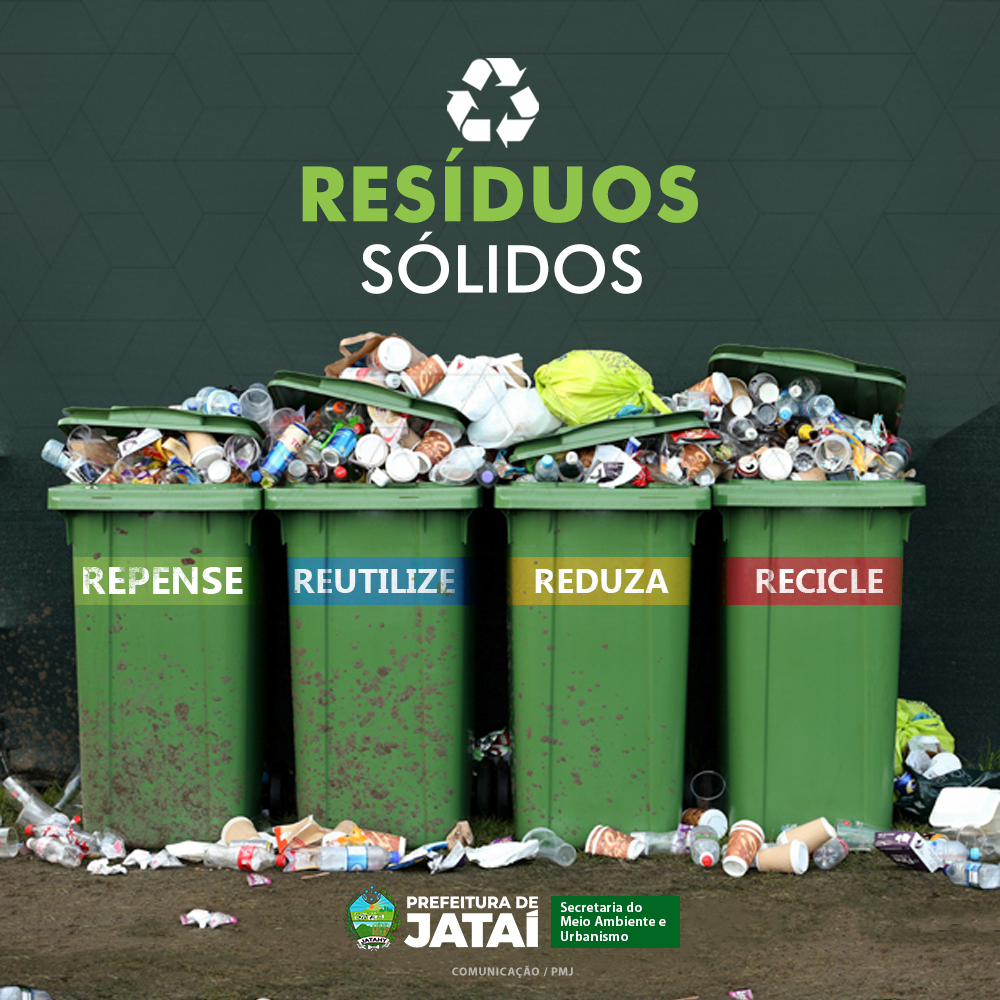
\includegraphics[width=5.90551in,height=5.90278in]{./imgSAEB_7_POR/media/image19.png}
\end{figure}

\fonte{Ulysses Gusmão de Oliveira e Luiz Carlos Pereira Borges.
Prefeitura de Jatái. Separe seu lixo de forma adequada. 
Disponível em: https://www.jatai.go.gov.br/separe-seu-lixo-de-forma-adequada/.
Acesso em: 2 out. 2023.}

Na imagem acima, são usados diversos recursos para que a mensagem
seja transmitida de maneira eficiente. No caso da escolha dos
verbos utilizados, é correto afirmar que:

\begin{escolha}

    \item as formas verbais no imperativo afirmativo sugerem ações.

    \item as formas verbais no infinitivo expressam instruções.

    \item as formas verbais no subjuntivo representam advertências.

    \item as formas verbais no infinitivo indicam ordens.

\end{escolha}

\num{15} Observe a imagem a seguir para responder à questão.

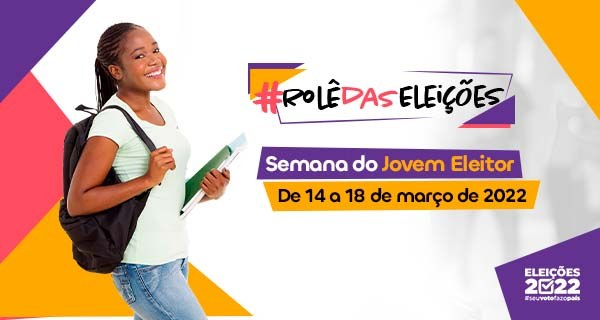
\includegraphics[width=5.90551in,height=3.15278in]{./imgSAEB_7_POR/media/image20.png}

% \fonte{Tribunal Regional Eleitoral de São Paulo. 
% Tuitaço #RolêdasEleições alcança trending topics no Twitter.
% Disponível em: https://www.tre-sp.jus.br/comunicacao/noticias/2022/Marco/tuitaco-roledaseleicoes-alcanca-trending-topics-no-twitter.
% Acesso em: 22 mai. 2023.}
\fonte{Tribunal Regional Eleitoral de São Paulo. 
Tuitaço \#RolêdasEleições alcança trending topics no Twitter.}

Pode-se afirmar que o público-alvo da campanha acima é

\begin{escolha}

    \item o público em geral, devido ao uso da linguagem formal combinada com imagens vivazes.
    
    \item o público adulto, daí a neutralidade sóbria do texto e a austeridade das imagens. 
    
    \item o público jovem, que se identificará com a imagem e que usa redes sociais.  
    
    \item a público infantil, pelo chamado lúdico do texto e das imagens à participação política. 

\end{escolha}


\chapter[Simulado 2]{Simulado}

\num{1} Leia o texto abaixo para responder à questão.

\begin{myquote}

No período entre julho e setembro, a ocorrência de queimadas se torna
mais frequente, por conta da estiagem e da baixa umidade relativa do ar.
A Especialista CNN em agronegócio Carmen Perez falou sobre as técnicas
empregadas nas fazendas para evitar que o fogo se alastre e cause
destruição.

Ela explicou que a seca traz dois principais alertas para produtores
rurais: a necessidade de garantir alimento aos animais e a atenção ao
risco de queimadas.``Cada fazenda tem diversas estratégias para coibir e
enfrentar incêndios'', explicou. Dentre elas, estão os aceiros, áreas
livres em que circulam parte da plantação para interromper a propagação do
fogo, reservatórios de água estratégicos e equipamentos específicos.

``Estamos no início da seca, mas já estamos alertas para evitar
possíveis riscos para a natureza, plantações e animais'', disse Perez.

\end{myquote}

% \fonte{Fernanda Pinotti. CNN Brasil. Carmen Perez: Fazendas têm diversas 
% estratégias para coibir incêndios. Disponível em:
% https://www.cnnbrasil.com.br/economia/carmen-perez-fazendas-tem-diversas-estrategias-para-coibir-incendios/
% Acesso em: 23 mai. 2023.}
\fonte{Fernanda Pinotti. CNN Brasil. Carmen Perez: Fazendas têm diversas 
estratégias para coibir incêndios.}

Segundo a especialista em agronegócio, qual fator requer maior atenção
dos produtores rurais no que diz respeito ao risco de queimadas?

\begin{escolha}
    
    \item As altas temperaturas.
    
    \item O período de estiagem.
    
    \item A alimentação dos animais.
    
    \item O descaso com questões ambientais.

\end{escolha}
  
\num{2} Leia o artigo 5 da Constituição Federal, de 1988, da República
Federativa do Brasil.

\begin{myquote}

Art. 5º Todos são iguais perante a lei, sem distinção de qualquer
natureza, garantindo-se aos brasileiros e aos estrangeiros residentes no
País, a inviolabilidade do direito à vida, à liberdade, à igualdade, à
segurança e à propriedade.

\end{myquote}

% \fonte{Presidência da República. Constituição da República Federativa do Brasil 
% de 1988. Disponível em: http://www.planalto.gov.br/ccivil_03/constituicao/constituicao.htm.
% Acesso em: 23 mai. 2023.}
\fonte{Presidência da República. Constituição da República Federativa do Brasil 
de 1988.}

A divisão em artigos caracteriza o trecho como:

\begin{escolha}

    \item O texto de uma lei.

    \item Uma carta de solicitação.

    \item Uma reivindicação.

    \item Uma petição.

\end{escolha}

\pagebreak

\num{3} Linguagem direta e curta, envolvendo poucos personagens, em espaço
delimitado e poucos conflitos e ações de personagens. Um texto que se
compõe de uma situação inicial, um conflito, clímax e desfecho. Estas
características estão presentes em:

\begin{escolha}

    \item Romance

    \item Contos

    \item Cartas pessoais

    \item Crônicas

\end{escolha}

\num{4} Leia o texto abaixo para responder à questão.

\begin{myquote}

Uma pesquisa realizada pelo Instituto de Estudos em Saúde Coletiva
(Iesc) e pela Faculdade de Medicina (FM), atualmente em revisão na
revista Scientific Reports, indicou que os programas sociais de
transferência de renda foram essenciais durante o período crítico da
covid-19. A investigação também ressaltou que a população negra teve um
maior índice de mortalidade no mesmo recorte temporal.

O estudo, que analisou dados de contágio da doença colhidos entre março
de 2020 e setembro de 2021 em todo o Brasil, detectou uma relação
inversa entre as taxas de mortalidade e infecção e o número de pessoas
de uma mesma família que eram beneficiárias de algum dos programas
governamentais.

\end{myquote}

% \fonte{Carol Correia. Conexão UFRJ. Programas sociais foram fundamentais durante fase crítica da covid-19.
% https://conexao.ufrj.br/2023/03/programas-sociais-foram-fundamentais-durante-fase-critica-da-covid-19/.
% Acesso em: 24 mai 2023.}
\fonte{Carol Correia. Conexão UFRJ. Programas sociais foram fundamentais durante fase crítica da covid-19.}

No texto acima, a linguagem objetiva e a apresentação de dados de pesquisa são traços do 
gênero:

\begin{escolha}

    \item artístico-literário.

    \item de divulgação científica.

    \item jornalístico midiático.

    \item jurídico.

\end{escolha}

\num{5} Leia o texto abaixo para responder à questão. 

\begin{myquote}

O livro \textit{A queda do Céu}, de Davi Kopenawa e Bruce Albert, é um modelo
inovador de produção textual, que combina a auto-etnografia de uma
cultura, o manifesto político das culturas tradicionais, os relatos de
vidas não ocidentais e uma visão cosmológica e espiritual do mundo,
quase extinta na sociedade moderna.

A obra retrata a vida do narrador (Kopenawa), desde sua iniciação
religiosa até alcançar o ápice como líder Yanomami.

Segundo sua cultura e tradições, os Yanomamis são os responsáveis por
assegurar que o céu não caia. Kopenawa, xamã da tribo, cita diversos
momentos em sua vida que exemplificam essas situações, onde ele ou os
antigos xamãs mobilizaram os espíritos para que a Floresta permanecesse
em equilíbrio.

\end{myquote}

% \fonte{Akil Alexandre Costa Silvério da Silva. Resenha do texto: \textit{A queda do Céu}: Davi Kopenawa e
% Bruce Albert. Disponível em: https://edisciplinas.usp.br/pluginfile.php/3395103/mod_resource/content/1/T6\%20aperfei\%C3\%A7oado.pdf.
% Acesso em: 24 mai. 2023.}
\fonte{Akil Alexandre Costa Silvério da Silva. Resenha do texto: \textit{A queda do Céu}: Davi Kopenawa e
Bruce Albert.}

No texto acima, notam-se características da

\begin{escolha}

    \item crônica (temas do cotidiano de forma crítica e bem humorada).

    \item resenha crítica (características e explicações de outra obra).

    \item notícia (informações ao leitor sobre fatos ocorridos).

    \item peça de teatro (texto escrito para ser encenado). 

\end{escolha}

\num{6} Leia o texto abaixo para responder à questão. 

\begin{myquote}

Na última década, o diabetes cresceu 54\% nos homens e 28,5\% nas
mulheres. Outra doença que tem crescido entre os brasileiros e que está
relacionada com o alto consumo de açúcar é a obesidade, que atinge
mais de 25\% da população adulta do país.

\end{myquote}

% \fonte{Ministério da Saúde. Saúde promove conscientização sobre o consumo de açúcar em webinário. 
% Disponível em: https://aps.saude.gov.br/noticia/15359\#:~:text=Os\%20brasileiros\%20consomem\%2050\%25\%20a,adulto\%20\%C3\%A9\%20de\%2012\%20colheres.
% Acesso em: 24 mai. 2023.}
\fonte{Ministério da Saúde. Saúde promove conscientização sobre o consumo de açúcar em webinário.}

De acordo com as informações acima, o consumo de açúcar pode ser
responsável pelos altos índices de obesidade. Além da obesidade, qual
outra doença pode estar relacionada ao consumo de açúcar? Assinale a
alternativa correta:

\begin{escolha}

  \item Diabetes.
  
  \item doenças crônicas não transmissíveis.
  
  \item doenças comuns em homens.
  
  \item doenças crônicas em mulheres. 

\end{escolha}

\num{7} Observe o meme abaixo para responder à questão.

%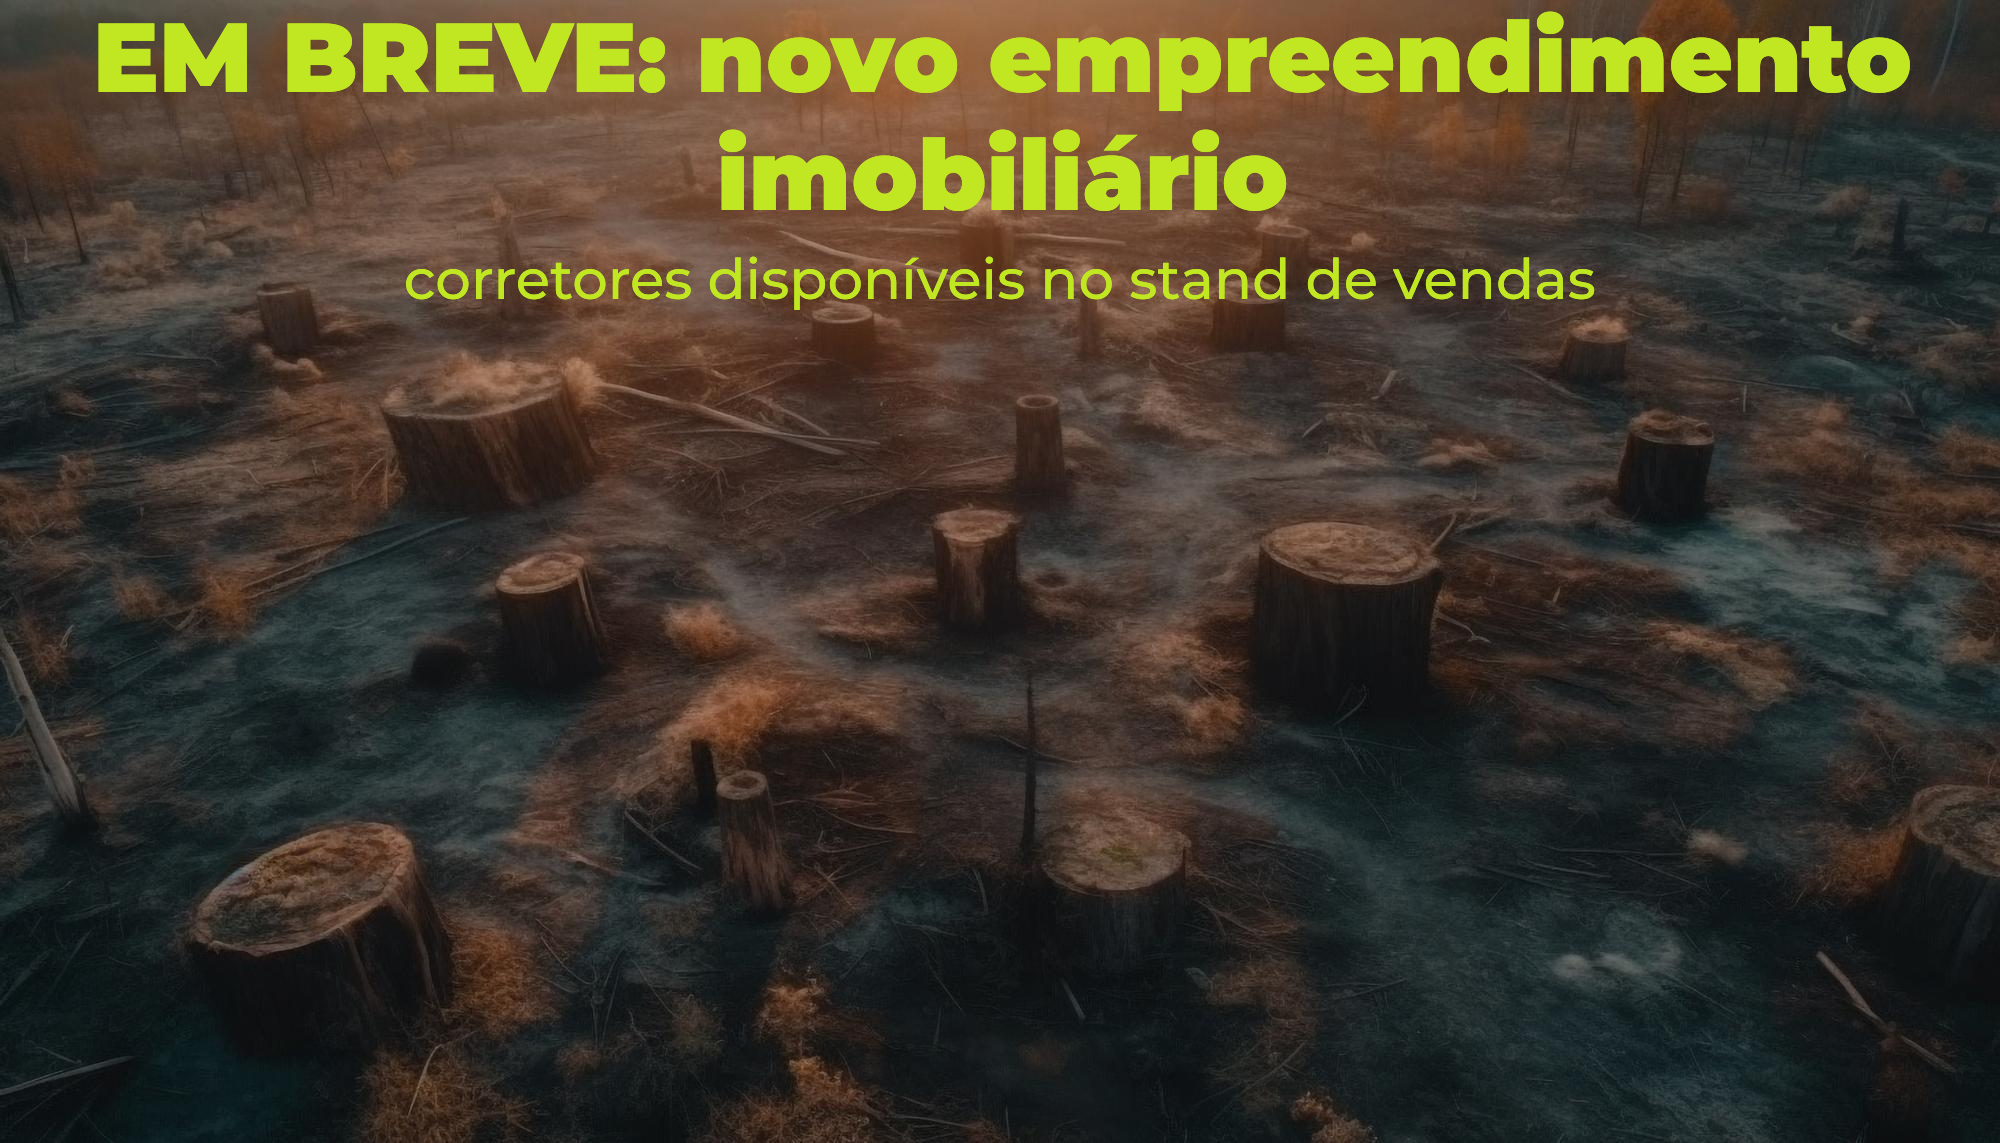
\includegraphics[width=4.16667in,height=3.03125in]{imgSAEB_7_POR/media/image21.png}

O efeito de sentido produzido pela imagem é bem claro. Assinale
alternativa que apresenta tais efeitos de sentido:

\begin{escolha}

    \item crítica ao desmatamento por meio de oposição.

    \item divulgação de informações por meio de imagem.

    \item persuasão por meio de frases injuntivas. 

    \item sensibilização por meio de frases motivacionais. 

\end{escolha}

\num{8} Leia o texto abaixo para responder à questão. 

\begin{myquote}

A teórica Kirin Narayan questiona esse dualismo e foca na qualidade das
relações que mantemos com as pessoas que buscamos representar em nossos
textos. Nesse sentido, a autora propõe desconstruir a ideia de que os
interlocutores poderiam ser classificados como meros indivíduos para
declarações acerca de um \textbf{``outro generalizado}'', impulsionando
assim um entendimento desses sujeitos como portadores de
\textbf{``vozes, perspectivas e dilemas''}.

\end{myquote}

% \fonte{Leonardo Bomfim. Desafios e potencialidades do ``pesquisador nativo'':
% perspectivas etnográficas em um festival musical.
% Disponível em: https://econtents.bc.unicamp.br/inpec/index.php/muspop/article/view/17627/12474.
% Acesso em: 24 mai. 2023.}
\fonte{Leonardo Bomfim. Desafios e potencialidades do ``pesquisador nativo'':
perspectivas etnográficas em um festival musical.}

Os termos destacados que aparecem entre aspas representam:

\begin{escolha}
    \item as falas do autor sobre o tema.

    \item ideias que devem ser reforçadas.

    \item partes principais do argumento.

    \item citação das palavras de Kirin Naryan.

\end{escolha}

\num{9} Leia o texto abaixo para responder à questão. 

\begin{myquote}

Falando sobre o jogo Minecraft, Pedro Rezende se consolidou como o
maior YouTuber de games do Brasil. ``A ideia inicial começou quando eu
precisava de ajuda para passar de uma fase em um jogo e procurei na
internet''. A fala é de um dos maiores youtubers da atualidade no Brasil. O jovem
paranaense Pedro Rezende (19) mudou sua vida da água para o vinho depois
que abandonou a profissão de goleiro em um time de futebol na Itália
para seguir a carreira de youtuber de games por aqui.

\end{myquote}

% \fonte{Jadson Falcão. A União. Geração de youtubers faz sucesso entre o público jovem. 
% Disponível em: https://auniao.pb.gov.br/noticias/caderno_diversidade/geracao-de-youtubers-faz-sucesso-entre-os-jovens-do-pais.
% Acesso em: 24 mai. 2023.}
\fonte{Jadson Falcão. A União. Geração de youtubers faz sucesso entre o público jovem.}

No contexto em que se insere, a expressão ``mudou sua vida da água para o vinho''
significa que 

\begin{escolha}

    \item a vida do garoto era miserável.

    \item o garoto trocou água por vinho.

    \item a vida do garoto continua a mesma.

    \item a vida do garoto mudou drasticamente.

\end{escolha}

\num{10} Leia o texto abaixo para responder à questão.

\begin{myquote}

\centering\textbf{``Ariel, a Pequena Sereia''"'' é opção de teatro para as crianças neste 
final de semana}

A programação cultural deste final de semana traz para o público infantil 
a peça teatral "Ariel, a Pequena Sereia". O espetáculo ganha sessões no Teatro 
Barreto Júnior, neste sábado (22) e domingo (23), às 16h30.

\end{myquote}

% \fonte{Folha de Pernambuco. 
% Disponível em:
% https://www.folhape.com.br/cultura/ariel-a-pequena-sereia-e-opcao-de-teatro-para-as-criancas-neste/267280/.
% Acesso em: 24 mai. 2023}
\fonte{Folha de Pernambuco.}

Na manchete e no corpo do texto as aspas foram usadas para

\begin{multicols}{2}
\begin{escolha}
    
    \item citar a fala de um entrevistado.
    
    \item citar o nome de uma obra,
    
    \item citar uma gíria.
    
    \item dar ênfase ao termo.

\end{escolha}
\end{multicols}

\num{11} Leia os textos abaixo para responder à questão. 

\begin{myquote}

\textbf{Texto 1}

Às 14h, ocorreu o acidente. Um desmoronamento interno fez com que uma
enorme rocha se desprendesse da montanha e caísse sobre o túnel,
fechando completamente a ligação com a superfície. Dentro da mina,
ficaram 33 mineiros -- 32 chilenos e 1 boliviano.

\end{myquote}

% \fonte{Rogério Simões. BBC News Brasil. 
% Mineiros do Chile: a incrível e dramática saga acompanhada pelo mundo ao vivo na TV.
% Disponível em: https://www.bbc.com/portuguese/internacional-55926799.
% Acesso em: 24 mai. 2023.}
\fonte{Rogério Simões. BBC News Brasil. 
Mineiros do Chile: a incrível e dramática saga acompanhada pelo mundo ao vivo na TV.}

\textbf{Texto 2}

\begin{myquote}

No dia 5 de agosto, um desmoronamento deixou 33 operários presos na mina
de San José, situada no deserto do Atacama, no Chile. Eles ficaram
incomunicáveis, a 700 metros de profundidade, durante 17 dias, até serem
descobertos pelas equipes de sondagem.

\end{myquote}

% \fonte{José Renato Salatiel. Mineiros do Chile: O resgate que emocionou o mundo.
% Disponível em: https://vestibular.uol.com.br/resumo-das-disciplinas/atualidades/mineiros-do-chile-o-resgate-que-emocionou-o-mundo.htm.
% Acesso em: 24 mai. 2023.}

\fonte{José Renato Salatiel. Mineiros do Chile: O resgate que emocionou o mundo.}

\renewcommand{\fonte}[1]{}

Assinale a única afirmação comum aos dois textos. 

\begin{escolha}

    \item O acidente ocorreu às 14 horas.

    \item O acidente deixou 33 operários presos.

    \item Os mineiros ficaram presos por 17 dias.

    \item O acidente atingiu 32 chilenos e 1 boliviano.

\end{escolha}

\num{12} Leia o texto abaixo para responder à questão. 

\begin{myquote}

\textbf{Nordeste poderia crescer mais que o Brasil até 2030}

Combinar aumento da produtividade com redução das desigualdades seria a
melhor alternativa para elevar o PIB per capita na região.

\fonte{Instituto de Pesquisa Econômica Aplicada. Nordeste poderia crescer mais
 que o Brasil até 2030. Disponível em:
 https://www.ipea.gov.br/portal/categorias/45-todas-as-noticias/noticia 9506-nordeste-poderia-crescer-mais-que-o-brasil-ate-2030?highlight=WyJub3JkZXN0ZSIsIm5vcmRlc3RlJy4iXQ==.
 Acesso em: 24 mai. 2023.}

\end{myquote}

De acordo com o texto, o Nordeste

\begin{escolha}
    
    \item vai crescer mais que o Brasil até 2030 e aumentar a produtividade para diminuir a desigualdade.
    
    \item só crescerá mais que o Brasil se combinar aumento da produtividade e redução da desigualdade. 
    
    \item já reduziu a desigualdade social e tem alcançado elevação proporcional do PIB.
    
    \item cresceu sensivelmente em relação ao Brasil, de modo que já conseguiu elevar o PIB.

\end{escolha}

\pagebreak

\num{13} Leia o texto abaixo para responder à questão. 

\begin{myquote}

Sua história tem pouca coisa de notável. Fora Leonardo
algibebe em Lisboa, sua pátria; aborrecera-se porém do negócio,
e viera ao Brasil. Aqui chegando, não se sabe por proteção de
quem, alcançou o emprego de que o vemos empossado, e que
exercia, como dissemos, desde tempos remotos. Mas viera com
ele no mesmo navio, não sei fazer o quê, uma certa Maria da
Hortaliça, quitandeira das praças de Lisboa, saloia rechonchuda e
bonitota. O Leonardo, fazendo-se-lhe justiça, não era nesse tempo
de sua mocidade mal apessoado, e sobretudo era maganão. Ao
sair do Tejo, estando a Maria encostada à borda do navio, o
Leonardo fingiu que passava distraído por junto dela, e com o
ferrado sapatão assentou-lhe uma valente pisadela no pé direito.
A Maria, como se já esperasse por aquilo, sorriu-se como
envergonhada do gracejo, e deu-lhe também em ar de disfarce um
tremendo beliscão nas costas da mão esquerda. Era isto uma
declaração em forma, segundo os usos da terra: levaram o resto
do dia de namoro cerrado; ao anoitecer passou-se a mesma cena
de pisadela e beliscão, com a diferença de serem desta vez um
pouco mais fortes; e no dia seguinte estavam os dois amantes tão
eXtremosos e familiares, que pareciam sê-lo de muitos anos.

\end{myquote}

\fonte{Manuel Antônio de Almeida. Memórias de um sargento de milícias.
 Disponível em: https://digital.bbm.usp.br/handle/bbm/1601. Acesso em: 24
 mai. 2023. 
Assinale a alternativa correta no que se refere à coesão e à coerência 
do texto.} 

\begin{escolha}

\item
  Em ``\textbf{Sua história} tem pouca coisa de notável'', o termo destacado
  se refere à história de Maria da Hortaliça.
\item
  Em ``assentou-\textbf{lhe} uma valente pisadela no pé direito'', o termo destacado
  se refere ao pé de Maria da Hortaliça.
\item
  Em ``deu-\textbf{lhe} também em ar de disfarce um tremendo beliscão'', o termo 
  destacado se refere ao pé de Maria da Hortaliça.
\item
  A expressão ``um pouco mais fortes'' refere-se à condição física de Leonardo e 
  Maria da Hortaliça.

\end{escolha}

\num{14} Leia o texto abaixo para responder à questão. 

\begin{myquote}

A vacina salva vidas. Doenças que causavam milhares de vítimas no
passado, como varíola e poliomielite, foram erradicadas. Outras doenças
transmissíveis também deixaram de ser problema de saúde pública porque
foram eliminadas no Brasil e nas Américas, como o sarampo, rubéola e
rubéola congênita.

\end{myquote}

\fonte{Ministério da Saúde. Programa Nacional de Imunizações -- Vacinação.
 Disponível em:
 https://www.gov.br/saude/pt-br/acesso-a-informacao/acoes-e-programas/programa-nacional-de-imunizacoes-vacinacao. Acesso em: 24 mai. 2023.}

Qual das seguintes opções melhor descreve a estratégia argumentativa
utilizada para enfatizar a importância da vacinação?

\begin{escolha}

    \item Emoção.
    
    \item Generalização.
    
    \item Lógica.
    
    \item Autoridade.

\end{escolha}

\num{15} Observe a imagem abaixo para responder à questão. 

\begin{myquote}


\includegraphics[width=5.90551in,height=3.18056in]{imgSAEB_7_POR/media/image22.png}

\fonte{https://www.tre-sp.jus.br/comunicacao/noticias/2022/Junho/campanha-201ctamo-junto201d-do-tre-sp-quer-incentivar-voto-consciente-dos-jovens.
 Acesso em: 24 mai. 2023.}

A imagem acima faz parte de uma campanha incentivando a votação. Ao analisar
as escolhas de linguagem utilizadas podemos afirmar que a campanha se dirige: 

\end{myquote}

\begin{escolha}

    \item ao público idoso.

    \item ao público infantil.

    \item a mulheres.

    \item ao público jovem.

\end{escolha}



% \begin{figure}
% \vspace*{-3cm}
% \hspace*{-3.7cm}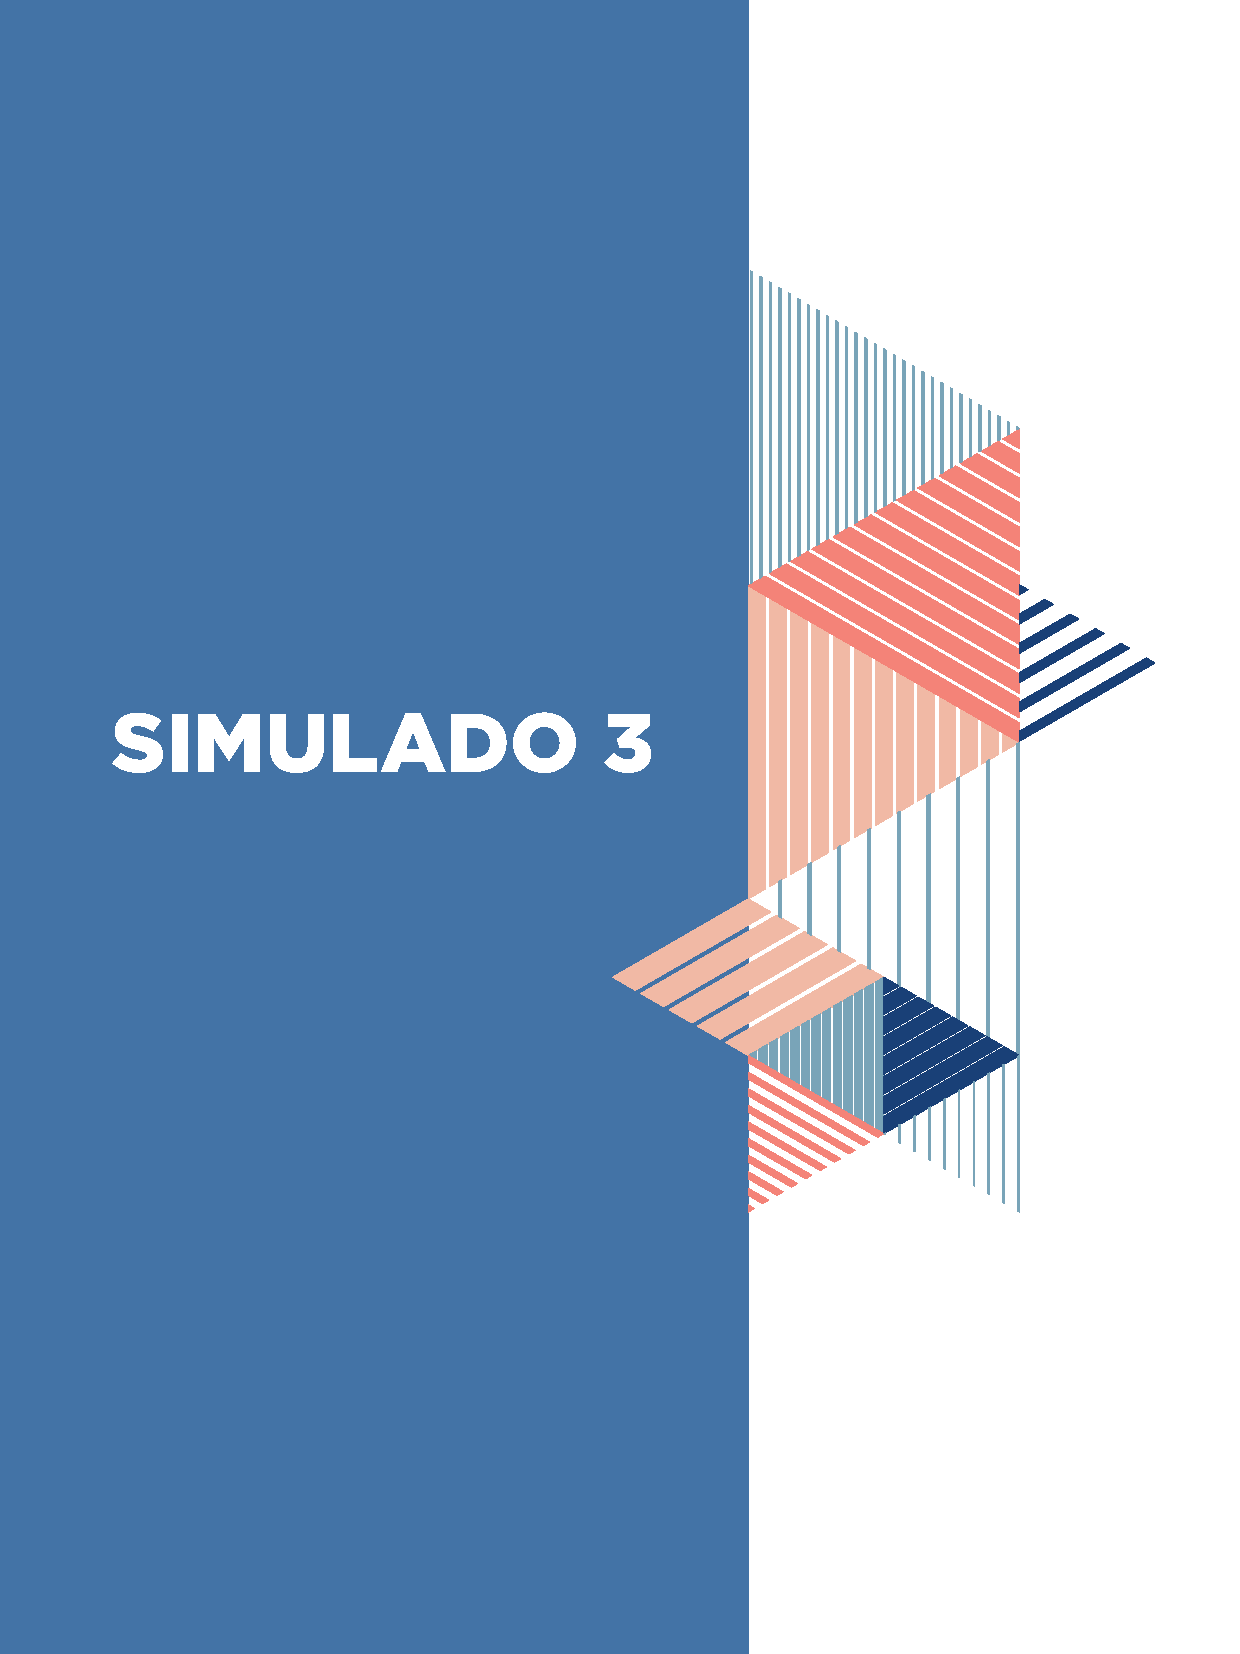
\includegraphics[scale=1]{../watermarks/3simulado9ano.pdf}
% \end{figure}


\chapter[Simulado 3]{Simulado}

\num{1} Leia o texto abaixo para responder à questão. 

\begin{myquote}

\textbf{Alimentos que prejudicam o meio ambiente são também os piores à
saúde}

\textit{Comer cereais, frutas, verduras, batatas e azeite de oliva protege o
planeta e previne doenças}

Aproximadamente 60\% dos fatores de risco responsáveis por todas as
doenças são o resultado de uma dieta de má qualidade. Esse fato está
ligado à saúde do planeta. Um estudo publicado na revista PNAS demonstra
que os alimentos mais prejudiciais ao ser humano também o são para a
Terra.

Os pesquisadores analisaram 15 alimentos que fazem parte da dieta diária
ocidental. Ligaram a maneira como são produzidos (a água que se gasta, a
superfície implicada e os produtos químicos utilizados, entre outros)
aos resultados de estudos anteriores sobre o impacto desses mesmos
alimentos sobre a saúde. E tudo se encaixava. As frutas, verduras, a
batata, o azeite de oliva, os legumes, as frutas secas e os cereais são
os alimentos mais saudáveis e que, além disso, têm impacto mínimo sobre
o planeta.

A carne vermelha processada e não processada, por outro lado, é um
produto que deveria sair da lista de compras.

O peixe é um dilema. É uma opção saudável, como a maioria das pessoas
sabe, mas tem uma pegada ambiental maior, ao lado do frango e dos
laticínios, do que as dietas baseadas em vegetais, de acordo com os
resultados do estudo. Basulto afirma que um produto é benéfico quando
impede o consumidor de comer alimentos mais prejudiciais para sua saúde.
``Se o cliente come peixe e não consome carne vermelha, portanto, é bom
para ele e para o planeta'', acrescenta.

\fonte{Agathe Cortes. El País Brasil. 
Disponível em: https://brasil.elpais.com/brasil/2019/10/29/ciencia/1572344750_688431.html.
Acesso em: 22 mai. 2023.}

\end{myquote}

Segundo a reportagem, assinale a alternativa que contém os alimentos
mais saudáveis e que menos impactam o planeta:

\begin{escolha}
  
    \item cereais, ovos, legumes.
  
    \item frutas, verduras, cereais.
  
    \item frutas, verduras, frango.
  
    \item frutas secas, azeite, carnes.

\end{escolha}

\num{2} Leia o texto abaixo para responder à questão. 

\begin{myquote}

No caso, a quantidade de comida industrializada ingerida parece
influenciar no aparecimento de doenças e na quantidade de mortes
prematuras. Esses estudos, no entanto, não conseguem demonstrar qual
seria o mecanismo por trás dessa aparente correlação.

A geriatra Claudia Suemoto, da Faculdade de Medicina da USP, que
coordenou o estudo do Elsa sobre ultraprocessados e desempenho
cognitivo, espera superar essa limitação em breve. Serão feitas imagens
do cérebro de voluntários para ver se o alto consumo de ultraprocessados
pode causar eventos isquêmicos ou pequenos derrames cerebrais, que, ao
longo do tempo, poderiam comprometer as funções cognitivas. ``Dessa
forma, poderemos investigar possíveis mecanismos que expliquem a
associação do ponto de vista estrutural'', conta Suemoto.

\end{myquote}

\pagebreak

Segundo o texto, a limitação a ser superada pela pesquisa é:

\begin{escolha}

    \item diminuir a quantidade de ingestão de ultraprocessados para evitar derrames e melhorar o desempenho cognitivo.

    \item impossibilidade de demonstrar o mecanismo por trás da relação entre o consumo de ultraprocessados e as mortes prematuras.
  
    \item conseguir imagens do cérebro de voluntários que sofreram derrame cerebral causado pelo consumo excessivo de ultraprocessados.
  
    \item estudar as funções cognitivas e os eventos isquêmicos de quem sofreu derrame cerebral causado pelo consumo excessivo de ultraprocessados.

\end{escolha}

\num{3} Leia o texto abaixo para responder à questão. 

\begin{myquote}

\textbf{Título I}

Das Disposições Preliminares

Art. 1º Esta Lei dispõe sobre a proteção integral à criança e ao
adolescente.

Art. 2º Considera-se criança, para os efeitos desta Lei, a pessoa até
doze anos de idade incompletos, e adolescente aquela entre doze e
dezoito anos de idade.

Parágrafo único. Nos casos expressos em lei, aplica-se excepcionalmente
este Estatuto às pessoas entre dezoito e vinte e um anos de idade.

\end{myquote}

\fonte{Presidência da República. 
Disponível em: https://www.planalto.gov.br/ccivil_03/leis/l8069.htm.
Acesso em: 24 mai. 2023.}

Estão presentes no texto acima e são características de textos legais ou
jurídicos

\begin{escolha}

\item linguagem impessoal e organização em títulos, capítulos e sessões.
\item uso de linguagem informal e organização em parágrafos e estrofes.
\item linguagem rebuscada e organização em títulos e subtítulos.
\item uso da primeira pessoa e organização em livre.
\end{escolha}

\num{4} Leia o texto abaixo para responder à questão. 

\begin{myquote}

\textbf{Faciap promove encontros para jovens empreendedores em Curitiba}

Entre quinta (25) e sexta-feira (26) acontecem dois eventos promovidos
pelos integrantes da ala jovem da Federação das Associações Comerciais e
Empresariais do Paraná (Faciap).

A Assembleia Geral Ordinária (AGO) da Confederação Nacional de Jovens
Empresários (Conaje), que começa nesta quinta-feira (25) é um evento
nacional e vai reunir jovens empreendedores de todo o Brasil. Já na
sexta-feira (26) acontece o Encontro Paranaense de Jovens
Empreendedores.

\end{myquote}

\fonte{CBN Curitiba. Faciap promove encontros para jovens empreendedores em Curitiba.
Disponível em: https://cbncuritiba.com.br/materias/faciap-promove-encontros-para-jovens-empreendedores-em-curitiba/.
Acesso em: 24 mai. 2023.}

Considerando os elementos constitutivos dos textos jornalísticos, a
informação sobre a cidade onde ocorre o evento está localizada:

\begin{multicols}{2}
\begin{escolha}
  
  \item no corpo da notícia.
  
  \item na lide.
  
  \item no título auxiliar.
  
  \item na manchete.

\end{escolha}
\end{multicols}

\num{5} Leia o poema abaixo para responder à questão. 

\begin{myquote}
\begin{verse}

Mas a minha tristeza é sossego \\
Porque é natural e justa \\
E é o que deve estar na alma \\
Quando já pensa que existe \\
E as mãos colhem flores sem ela dar por isso.

\end{verse}
\end{myquote}

\fonte{Alberto Caeiro (heterônimo de Fernando Pessoa. O Guardador de Rebanhos. 
Disponível em: http://www.dominiopublico.gov.br/download/texto/pe000001.pdf.
Acesso em: 24 mai. 2023.}

Pode-se inferir que, para o eu lírico do poema, sua tristeza

\begin{escolha}

    \item causa confusão ao colher as flores.

    \item impede que a justiça natural ocorra.

    \item repousa distante dele mesmo. 

    \item traz quietude por ser natual e justa. 

\end{escolha}

\num{6} Leia o texto abaixo para responder à questão. 

%Excluí essa imagem
%
\includegraphics[width=5.90551in,height=1.70833in]{imgSAEB_7_POR/media/image3.png}
%\fonte{https://tirasarmandinho.tumblr.com/}{{https://tirasarmandinho.tumblr.com/}}.
%Acesso em 26 de Abr de 2023

\begin{myquote}

Dito isto, expirei às duas horas da tarde de uma
sexta-feira do mês de agosto de 1869, na minha bela
chácara de Catumbi. Tinha uns sessenta e quatro anos,
rijos e prósperos, era solteiro, possuía cerca de trezentos
contos e fui acompanhado ao cemitério por onze amigos.
Onze amigos! Verdade é que não houve cartas nem
anúncios. Acresce que chovia -- peneirava uma chuvinha
miúda, triste e constante, tão constante e tão triste \ldots{}

\end{myquote}

\fonte{Machado de Assis. Memórias Póstumas de Brás Cubas. 
Disponível em: https://digital.bbm.usp.br/handle/bbm/4826.
Acesso em: 24 mai. 2023.}

Nos dois últimos períodos do parágrafo, o narrador pretende 

\begin{escolha}

    \item justificar o pequeno número de presentes a seu enterro. 

    \item lamentar a injustiça de ter morrido cedo e com saúde.

    \item exaltar a popularidade que tinha entre os amigos.

    \item agradecer sinceramente aos amigos que o acompanharam.

\end{escolha}

\num{7} Leia o texto. 


\begin{myquote}

\textit{Câncer de mama}
É o tipo de câncer mais frequente na mulher brasileira. Nesta doença,
ocorre um desenvolvimento anormal das células da mama, que
multiplicam-se repetidamente até formarem um tumor maligno.

\textit{Como descobrir a doença mais cedo?}
Toda mulher com 40 anos ou mais de idade deve procurar um ambulatório,
centro ou posto de saúde para realizar o exame clínico das mamas
anualmente, além disso, toda mulher, entre 50 e 69 anos deve fazer pelo
menos uma mamografia a cada dois anos. O serviço de saúde deve ser
procurado mesmo que não tenha sintomas!

\textit{O que é o exame clínico das mamas?}
É o exame das mamas realizado por médico ou enfermeiro treinado para
essa atividade. Neste exame poderão ser identificadas alterações nas
mesmas. Se for necessário, será indicado um exame mais específico, como
a mamografia.

\textit{O auto-exame previne a doença?}
O exame das mamas realizado pela própria mulher, apalpando os seios,
ajuda no conhecimento do próprio corpo, entretanto, esse exame não
substitui o exame clínico das mamas realizado por um profissional de
saúde treinado. Caso a mulher observe alguma alteração deve procurar
imediatamente o serviço de saúde mais próximo de sua residência. Mesmo
que não encontre nenhuma alteração no auto-exame, as mamas devem ser
examinadas uma vez por ano por um profissional de saúde!

\end{myquote}

\fonte{Biblioteca Virtual em Saúde. Câncer de mama. Disponível em:
https://bvsms.saude.gov.br/cancer-de-mama/.
Acesso em: 24 mai. 2023.}

O que faz com que as
informações sejam confiáveis é a presença de

\begin{escolha}
    
    \item textos explicativos.
    
    \item imagens e textos.
    
    \item citação de fontes oficiais.
    
    \item linguagem clara.

\end{escolha}

\num{8} Leia o texto abaixo para responder à questão. 

\begin{myquote}

\textbf{O que a ciência diz sobre os remédios naturais para dormir}

\textit{Se você tomar um chazinho à base de ervas ou borrifar o quarto com
aromas agradáveis... será que vai conseguir dormir como um bebê?}

O sono raramente é mais desejado do que quando não conseguimos dormir.

E há uma grande variedade de remédios caseiros que prometem nos ajudar a
pegar no sono sem recorrer a produtos farmacêuticos.

\end{myquote}

\fonte{G1. Disponível em: https://g1.globo.com/saude/noticia/2023/04/26/o-que-a-ciencia-diz-sobre-os-remedios-naturais-para-dormir.ghtml. 
Acesso em: 24 mai. 2023.}

A expressão ``raramente'', para se referir ao desejo de dormir, expressa:

\begin{escolha}
  
  \item que o sono é mais desejado quando não se consegue dormir.
  
  \item que na maioria das vezes o sono é desejado em qualquer ocasião.
  
  \item que sempre sentimos sono quando precisamos dormir.
  
  \item que só sentimos sono quando não desejamos dormir. 

\end{escolha}

\num{9} Leia o texto abaixo para responder à questão. 

\begin{myquote}

\textbf{-- Por que não ser também um chato?}

\begin{verse}

Mas de repente percebi \\
Sem ser doutor \\
Que a chatice é a única doença \\
que não dói no portador \\
E resolvi ser chato. 

\end{verse}
\end{myquote}

\fonte{Millor Fernandes. Poeminha Maçante, no livro Circo de palavras: histórias, poemas, pensamentos.
São Paulo: Ática, 2007. p. 63.}

Segundo o poema, o eu lírico escolheur ser chato porque 

\begin{escolha}

  \item a chatice é uma doença.
  
  \item ser chato não dói.
  
  \item ele queria ser doutor.
  
  \item se percebeu chato de repente.

\end{escolha}

\num{10} Leia o texto abaixo para responder à questão. 

\begin{myquote}

O casamento fez-se onze meses depois, e foi a mais bela festa das
relações dos noivos. Amigas de Clara, menos por amizade que por
inveja, tentaram arredá-la do passo que ia dar. Não negavam a gentileza
do noivo, nem o amor que lhe tinha, nem ainda algumas virtudes; diziam
que era dado em demasia a patuscadas.

\end{myquote}

\fonte{Machado de Assis. Pai contra mãe. 
Disponível em: http://www.dominiopublico.gov.br/download/texto/bv000245.pdf.
Acesso em: 24 mai. 2023.}

De acordo com o texto, as amigas de Clara

\begin{escolha}

    \item tentaram impedir o casamento dela porque lhe nutriam amizade honesta.

    \item persuadiram-na a desistir por causa da falsidade dos sentimentos do noivo.  

    \item desaprovavam o casamento porque não lhe nutriam amizade verdadeira.

    \item tentaram convencê-la a desistir do casamento por inveja, apesar da amizade.

\end{escolha}

\num{11} Observe os períodos a seguir.

\begin{itemize}

    \item \textbf{Já que} o vento soprava muito forte, decidiram não sair
naquela noite.

    \item Eu não consegui ir ao escritório \textbf{porque} estava muito doente

    \item Os jovens terão suas necessidades ouvidas, \textbf{exceto} se se
afastarem dos responsáveis.

    \item \textbf{Embora} estivesse triste, não chorou.

\end{itemize}

Assinale a alternativa que indica corretamente as relações de sentido
expressas pelos conectivos em destaque.

\begin{escolha}

    \item causa, causa, condição, concessão.

    \item comparação, condição, finalidade, oposição.

    \item causa, oposição, condição, finalidade

    \item finalidade, comparação, tempo, causa.

\end{escolha}

\num{12} Leia o texto abaixo para responder à questão. 

\begin{myquote}

Em relação ao consumo de agrotóxicos no Brasil, hoje paira uma grande
incerteza sobre os números exatos. No ano de 2015, só foram divulgados
os valores em dólares dos ganhos da indústria. Neste sentido, houve uma
forte queda, de 21\%, em relação a 2014. No entanto, se considerarmos a
variação do câmbio, vemos que na verdade o faturamento em reais subiu de
R\$28 para R\$32 bilhões. Como uma boa parte do custo dos agrotóxicos é
importada, não é possível saber se aumentou ou diminuiu a quantidade de
agrotóxicos em 2015.

\end{myquote}

\fonte{Alan Tygel. Agrotóxicos no Brasil: O veneno ainda está na mesa.  
Disponível em:
https://www.brasildefato.com.br/2016/11/23/agrotoxicos-no-brasil-o-veneno-ainda-esta-na-mesa.
Acesso em: 24 mai. 2023.}

Assinale a alternativa que contém a figura de linguagem correta e o
trecho em que essa figura aparece.

\begin{escolha}

    \item Hipérbole em ``Agrotóxicos do Brasil''. 

    \item Metáfora em ``hoje paira uma grande incerteza sobre os números exatos''. 

    \item Metonímia em ``O veneno ainda está na mesa''. 

    \item Hipérbole em ``Neste sentido, houve uma forte queda, de 21\%''. 

\end{escolha}

\num{13} Leia o texto abaixo para responder à questão. 

\begin{myquote}

Uma noite destas, vindo da cidade para o Engenho
Novo, encontrei no trem da Central um rapaz aqui do
bairro, que eu conheço de vista e de chapéu. 
Cumprimentou-me, sentou-se ao pé de mim, falou da lua
e dos ministros, e acabou recitando-me versos. A viagem 
era curta, e os versos \textbf{pode ser que não fossem} 
inteiramente maus. Sucedeu, porém, que, como eu estava 
cansado, fechei os olhos três ou quatro vezes; tanto 
bastou para que ele interrompesse a leitura e metesse 
os versos no bolso.

\end{myquote}

\fonte{Machado de Assis. Dom Casmurro. 
Disponível em: https://www.ic.unicamp.br/~stolfi/misc/2012-02-13-domine-casmurrus.pdf.
Acesso em: 24 mai. 2023.}

A escolha dos verbos no trecho em destaque dá a entender que o narrador

\begin{escolha}

  \item julga ruins os versos do rapaz e interrompe-lhe a leitura.

  \item considera bons os versos do rapaz, apesar de cansativos.

  \item não tolera a falta de qualidade da poesia do rapaz.

  \item avalia que os versos não eram ruins, sem considerá-los bons.

\end{escolha}

\num{14} Leia o texto abaixo para responder à questão. 

\begin{myquote}

\textbf{Os cosplays mais irados de 2021}

Apesar da pandemia, a criatividade na cultura pop não parou,
por isso vamos ver os cosplays que mais se destacaram em 2021 até
agora!

\end{myquote}

\fonte{Terra. Os cosplays mais irados de 2021. 
Disponível em: https://www.terra.com.br/gameon/geek/os-cosplays-mais-irados-de-2021,b409f1697bb7db34500d0614340e6423966k7p1p.html.
Acesso em: 24 mai. 2023.}

No exemplo acima, observam-se algumas variações linguísticas. Assinale a
alternativa que contém a correta descrição de termos do texto.

\begin{escolha}
  
  \item cosplays: estrangeirismo.
  
  \item cultura pop: regionalismo.
  
  \item irados: norma-padrão.
  
  \item criatividade: gíria.

\end{escolha}

\num{15} Leia o texto abaixo para responder à questão. 

\begin{myquote}

\textbf{Os ``causos'' de Joseli Dias}

O ofício de jornalista de Joseli Dias deu-lhe a agilidade de lidar com
as palavras. As narrativas das lendas e dos ``causos'' desta região,
reunidas no livro \textit{Mitos e Lendas do Amapá}, se constituem em um trabalho
de suma importância para todos nós, que valorizamos os elementos mais
puros e autênticos da nossa cultura popular.

\fonte{Joseli Dias. Mitos e lendas no Amapá. 
Disponível em: https://www2.senado.leg.br/bdsf/bitstream/handle/id/576836/Mitos_lendas_Amapa.pdf.
Acesso em: 24 mai. 2023.}

\end{myquote}

O uso do termo ``causos'' se justifica, pois, nos textos de Joseli Dias,

\begin{escolha}
    
    \item era necessário o uso da linguagem formal para retratar os mitos da região do Amapá..
    
    \item o ofício do jornalismo impunha a seu estilo a objetividade breve dos cronistas.
    
    \item as gírias da juventude de sua época ganham expressão literária significativa.
    
    \item a pureza e a autenticidade da cultura popular se manifestam por meio do vocabulário.

\end{escolha}

% \begin{figure}
% \vspace*{-3cm}
% \hspace*{-3.7cm}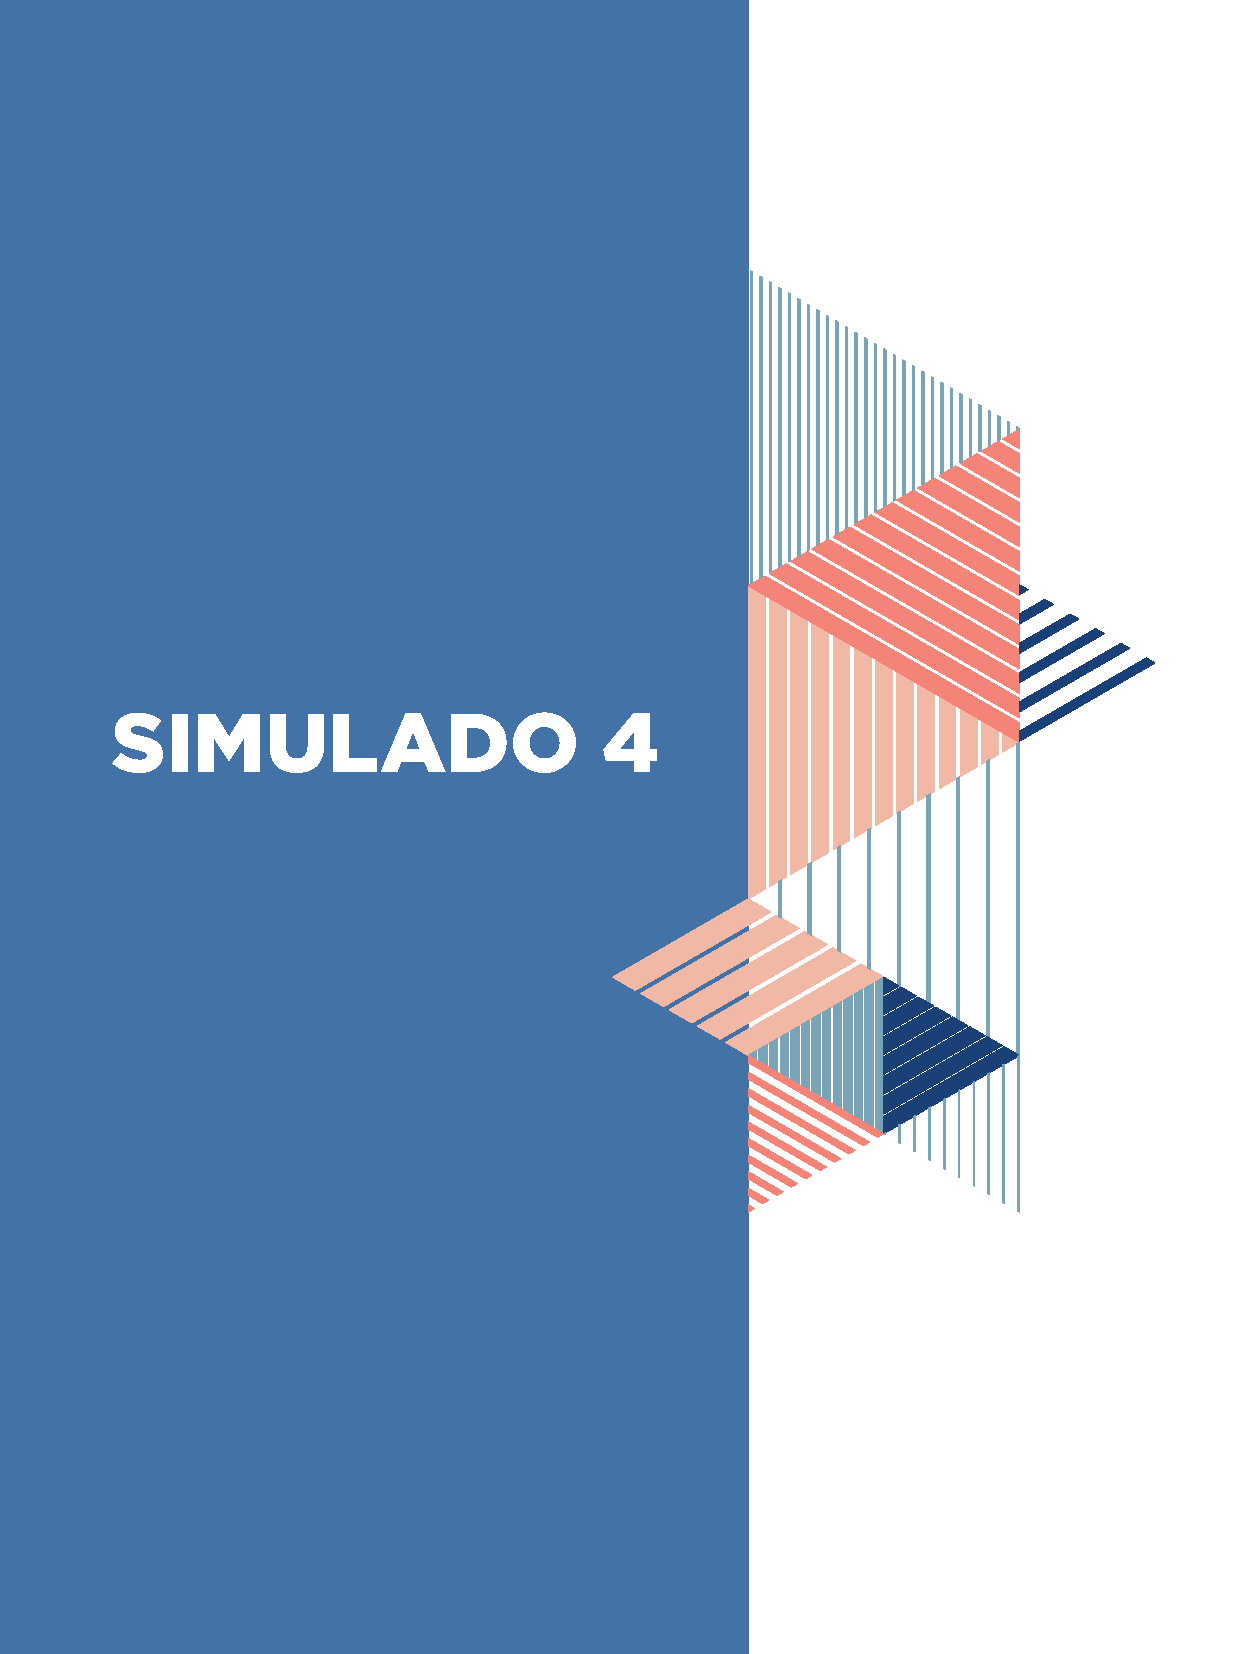
\includegraphics[scale=1]{../watermarks/4simulado9ano.pdf}
% \end{figure}

\chapter[Simulado 4]{Simulado}

\num{1} Leia o texto a seguir para responder à questão. 

\begin{myquote}

\textbf{França limitará o aumento do preço da eletricidade até 2025}

\textit{Recuperação da atividade econômica após a pandemia do coronavírus
provocou uma alta nos preços da energia na Europa}

A França vai prolongar até 2025 os subsídios adotados em outubro de 2021
para limitar o aumento do preço da eletricidade, em um contexto de
preocupação com a perda de poder de compra, anunciou o governo nesta
sexta-feira (21).

Le Maire alertou, por outro lado, que encerrará este ano o programa para
limitar o aumento dos preços do gás, já que estes ``voltaram ao nível
anterior à crise, de 50 euros por megawatt-hora''.

A recuperação da atividade econômica após a pandemia do coronavírus
provocou uma alta nos preços da energia na Europa no final de 2021, que
disparou meses depois com o início da invasão russa à Ucrânia.

\end{myquote}

\fonte{Folha de Pernambuco. França limitará o aumento do preço da eletricidade 
até 2025
Disponível em:
https://www.folhape.com.br/noticias/franca-limitara-o-aumento-do-preco-da-eletricidade-ate-2025/267267/.
Acesso em: 24 mai. 2023.}

Segundo a matéria os aumentos do preço da energia se devem:

\begin{escolha}
    
    \item à recuperação econômica pós pandemia e falta economia dos franceses.
    
    \item ao programa do governo que se encerra.
    
    \item à recuperação da atividade econômica e à guerra na Ucrânia.
    
    \item à preocupação com o poder de compra dos franceses.

\end{escolha}

\pagebreak

\num{2} Leia o texto abaixo para responder à questão. 


\begin{figure}[H]
\centering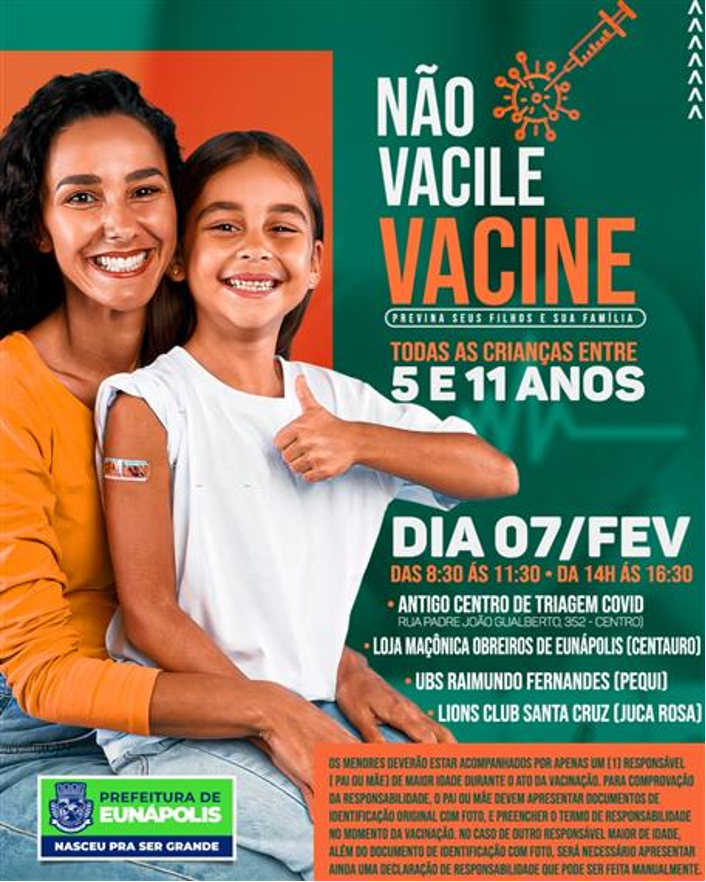
\includegraphics[width=.5\textwidth]{imgSAEB_7_POR/media/image24.png}
%\fonte{Prefeitura Municipal de Eunápolis. Vacinação: Covid-19 para crianças de 5 a 11 anos. 
%Disponível em: https://www.eunapolis.ba.gov.br/site/Noticias/noticia-060220221925071633-Vacina-o-Covid-19-para-crian-as-de-5-a-11-anos.
%Acesso em: 24 mai. 2023.}
\end{figure}



A força expressiva da campanha acima advém sobretudo 

\begin{escolha}
    
    \item da imagem inesperada que ilustra o cartaz.
    
    \item do contraste entre as cores de fundo. 
    
    \item do destaque da lista de locais de vacinação. 
    
    \item do jogo de palavras em ``não vacile, vacine''.

\end{escolha}

\num{3} Leia o texto abaixo para responder à questão. 

\begin{myquote}

CAPÍTULO I

DISPOSIÇÕES GERAIS

Art. 1º É instituída a Lei Brasileira de Inclusão da Pessoa com
Deficiência (Estatuto da Pessoa com Deficiência), destinada a assegurar
e a promover, em condições de igualdade, o exercício dos direitos e das
liberdades fundamentais por pessoa com deficiência, visando à sua
inclusão social e cidadania.

Parágrafo único. Esta Lei tem como base a Convenção sobre os Direitos
das Pessoas com Deficiência e seu Protocolo Facultativo, ratificados
pelo Congresso Nacional por meio do Decreto Legislativo nº 186, de 9 de
julho de 2008 , em conformidade com o procedimento previsto no § 3º do
art. 5º da Constituição da República Federativa do Brasil , em vigor
para o Brasil, no plano jurídico externo, desde 31 de agosto de 2008, e
promulgados pelo Decreto nº 6.949, de 25 de agosto de 2009 , data de
início de sua vigência no plano interno.

\end{myquote}

\fonte{Presidência da República. 
Lei Brasileira de Inclusão da Pessoa com Deficiência (Estatuto da Pessoa com Deficiência).
Disponível em: https://www.planalto.gov.br/ccivil_03/_ato2015-2018/2015/lei/l13146.htm.
Acesso em: 24 mai. 2023.}

O texto acima pertence ao domínio dos textos normativos e tem como
objetivo assegurar os direitos das pessoas com deficiência. Esta
afirmação pode ser comprovada pelo

\begin{escolha}
    
    \item artigo primeiro das disposições gerais.
    
    \item artigo quinto da Constituição Federal.
    
    \item capítulo I.
    
    \item parágrafo único.

\end{escolha}

\num{4} Leia o texto abaixo para responder à questão. 

\begin{myquote}

Aqui em Manaus faço uma parte desse grande projeto que é desenvolvido
por diversas instituições japonesas e conta com financiamento da GHIT
Funding, tendo à frente o doutor Shigeto Yoshida, da Universidade de
Kanazawa, no Japão, que é o desenvolvedor dessa formulação vacinal.
Essa vacina atua contra o parasita no hospedeiro humano e, também,
tentando evitar a infecção do hospedeiro que é o vetor, que transmite a
doença de uma pessoa para outra. Ela tem na sua forma a proteína CSP,
presente na vacina que já está em uso em diversos países da África e na
vacina desenvolvida pela Universidade de Oxford, no Reino Unido. Então
ela tem esse pedaço do parasita, essa proteína, que é um alvo estudado
já há muitos anos e com poder de proteção para as infecções nos humanos.
Essa proteína tem um papel importante para impedir que o parasita chegue
ao fígado, que é o primeiro local em que ele se instala, e, por causa
disso, os anticorpos e a resposta celular produzidos por uma vacina
poderiam impedir a entrada do parasita e seu desenvolvimento nos
humanos.

\end{myquote}

\fonte{Ciça Guedes. Ciência Hoje. Malária: uma vacina contra um desafio amazônico.
Disponível em: https://cienciahoje.org.br/artigo/malaria-uma-vacina-contra-um-desafio-amazonico/
Acesso em: 24 mai. 2023.}

Neste texto, podemos ver a explicação de como devem funcionar as vacinas
contra a malária e como estão sendo desenvolvidas. Assinale a alternativa
cuja expressão destacada seja marcador discursivos de causa.

\begin{escolha}

    \item \ldots ``conta com financiamento da GHIT Funding, \textbf{tendo à frente} o doutor Shigeto Yoshida''.

    \item ``\textbf{e, também}, tentando evitar a infecção do hospedeiro''.

    \item ``\textbf{Então} ela tem esse pedaço do parasita''.

    \item ``e, \textbf{por causa disso}, os anticorpos e a resposta celular''.

\end{escolha}

\num{5} Leia os textos abaixo para responder à questão. 

\begin{myquote}

\textbf{Exemplo 1}

A relação do ser humano com os animais de estimação existe há mais de 10
mil anos. Os animais domésticos preenchem várias necessidades emocionais
dos homens e dessa forma esses bichinhos, principalmente cães e gatos,
se tornam cada vez mais parte da nossa casa e de nossa família.

Mas infelizmente, muita gente ainda possui animais de estimação, mas não
possui a menor condição de criá-los. E quando falamos em condição de
criar, refiro-me principalmente a condições psicológicas.

Tanto é verdade que os maus-tratos aos ``pets'' são evidentes em todas as
cidades do país: animais famintos, torturados, feridos covardemente,
confinados em espaços minúsculos ou abandonados nas ruas ou estradas
Brasil afora.

E se quisermos mudar essa situação, precisamos perder o medo e o receio
de nos envolver e denunciar os maus-tratos, que só cessarão
quando aqueles que cometem esses crimes começarem a ser exemplarmente
punidos.

\end{myquote}

\fonte{Hugo Xavier. Jornal Cidade. Os maus tratos e o abandono de animais. 
Disponível em: https://www.jornalcidademg.com.br/artigo-os-maus-tratos-e-o-abandono-de-animais/. 
Acesso em: 24 mai. 2023.}

\textbf{Exemplo 2}

\begin{myquote}

\textbf{Polícia resgata 10 cachorros em situação de maus-tratos em dois
imóveis de Curitiba}

Resgate aconteceu no bairro Abranches e no Barreirinha. Polícia chegou
aos casos após denúncias de vizinhos.

A Polícia Civil e a Rede de Proteção Animal de Curitiba resgataram 10
cachorros que estavam em situação de maus-tratos na capital paranaense,
na quinta-feira (23).

O resgate aconteceu em dois imóveis, um no bairro Abranches e outro no
Barreirinha.

O proprietário do imóvel do Abranches foi multado em R\$ 12 mil, por
criação e venda irregulares e maus-tratos aos animais. A suspeita é que
no local existia um criadouro ilegal.

\end{myquote}

\fonte{G1. Polícia resgata 10 cachorros em situação de maus-tratos em dois imóveis de Curitiba.
Disponível em: https://g1.globo.com/pr/parana/noticia/2023/02/24/policia-resgata-10-cachorros-em-situacao-de-maus-tratos-em-dois-imoveis-de-curitiba.ghtml
Acesso em: 24 mai. 2023.}

Os dois exemplos foram extraídos de meios de comunicação e representam
diferentes gêneros do campo jornalístico. Com base nas diferenças entre
os dois textos é correto afirmar que:

\begin{escolha}
    
    \item O Exemplo 1 é uma entrevista e o Exemplo 2 é uma notícia.
    
    \item O Exemplo 1 é um artigo de opinião e o Exemplo 2 uma notícia.
    
    \item O Exemplo 1 é uma reportagem e o Exemplo 2 um artigo de opinião.
    
    \item O Exemplo 1 é uma carta de leitor e o Exemplo 2 é um artigo de opinião.

\end{escolha}

\num{6} Leia o soneto abaixo para responder à questão. 

\begin{myquote}
\begin{verse}

Apartava-se Nise de Montano, \\
em cuja alma partindo se ficava; \\
que o pastor na memória a debuxava, \\
por poder sustentar-se deste engano.

Pelas praias do Índico Oceano \\
sobre o curvo cajado se encostava, \\
e os olhos pelas águas alongava, \\
que pouco se doíam de seu dano.

Pois com tamanha mágoa e saudade \\
(dizia) quis deixar me a que eu adoro, \\
por testemunhas tomo Céu e estrelas.

Mas se em vós, ondas, mora piedade, \\
levai também as lágrimas que choro, \\
pois assim me levais a causa delas!

\end{verse}
\end{myquote}

\fonte{Luís de Camões. Sonetos.  
Disponível em: http://www.dominiopublico.gov.br/download/texto/bv000164.pdf.
Acesso em: 24 mai. 2023.}

Considerando os elementos que caracterizam os textos literários, o texto
acima pode ser considerado

\begin{escolha}

    \item conto, com personagens de ações restritas a espaço limitado.
    
    \item texto dramático, com falas de personagens e rubricas.  
    
    \item poema, baseado na sonoridade de versos divididos em estrofes.  
    
    \item romance, extensa narração de ações de diversos conflitos. 

\end{escolha}

\num{7} Leia o texto abaixo para responder à questão. 

\begin{myquote}

\textbf{Falta de iluminação em rua completa 1 ano e tem ``festa de
aniversário'' como protesto em Ourinhos}

Manifestação foi na Rua Narciso Nicolosi, no Jardim Paulista. Prefeitura
informou na manhã seguinte ao ato que fez a troca de lâmpada queimada.

Moradores de Ourinhos (SP) protestaram contra a falta de iluminação
pública na Rua Narciso Nicolosi, no Jardim Paulista, na noite desta
quarta-feira (26) com uma ``festa de aniversário'' para marcar um ano de
espera pela troca de lâmpadas em um poste.

A ``comemoração'' teve bolo com vela, refrigerante, bexigas, cartazes e
parabéns para você em coro e palmas em meio a críticas pela escuridão.

\end{myquote}

\fonte{G1. Falta de iluminação em rua completa 1 ano e tem 'festa de 
aniversário' como protesto em Ourinhos. 
Disponível em: https://g1.globo.com/sp/bauru-marilia/noticia/2023/04/27/falta-de-iluminacao-em-rua-completa-1-ano-e-tem-festa-de-aniversario-como-protesto-em-ourinhos.ghtml.
Acesso em: 24 mai. 2023.}

Os termos entre aspas na notícia expressam

\begin{escolha}
    
    \item ironia. 
    
    \item citação de falas de autoridades da cidade.
    
    \item citação de argumentos de especialistas.
    
    \item enfase nas palavras e termos destacados.

\end{escolha}

\num{8} Leia o texto abaixo para responder à questão. 

\begin{myquote}

\textbf{Telegram diz que Justiça ordenou entrega de dados ``impossíveis''
de serem obtidos; PF afirma que lentidão permitiu exclusão de
informações}

\textit{Cofundador do aplicativo afirmou que empresa está recorrendo da
suspensão do serviço, que começou a valer na noite da última quarta
(26).}

O cofundador do Telegram Pavel Durov afirmou nesta quinta-feira (27) que
a Justiça brasileira ordenou a entrega de dados ``impossíveis'' de serem
coletados. Em seu canal no aplicativo, ele afirmou que a empresa vai
recorrer da decisão.

\end{myquote}

\fonte{G1. Telegram diz que Justiça ordenou entrega de dados impossíveis 
de serem obtidos; PF afirma que lentidão permitiu exclusão de informações. 
Disponível em: https://g1.globo.com/tecnologia/noticia/2023/04/27/telegram-diz-que-justica-ordenou-coleta-de-dados-impossiveis-de-serem-obtidos-pf-afirma-que-lentidao-permitiu-exclusao-de-informacoes.ghtml.
Acesso em: 24 mai. 2023.}

Considerando a notícia acima, pode-se afirmar que o título da notícia expressa

\begin{escolha}

    \item concordância do autor com a justificativa da empresa. 

    \item simpatia do autor pela decisão da Polícia Federal.  

    \item intenção de influenciar a opinião do leitor.  

    \item tentativa de apresentar dois pontos de vista opostos. 

\end{escolha}

\num{9} Leia o texto abaixo para responder à questão. 

\begin{myquote}

\textbf{O rato do mato e o rato da cidade}

Um ratinho da cidade foi uma vez convidado para ir à casa
de um rato do campo. Vendo que seu companheiro vivia pobremente de
raízes e ervas, o rato da cidade convidou-o a ir morar com ele:

-- Tenho muita pena da pobreza em que você vive --
disse. -- Venha morar comigo na cidade e você verá como lá a
vida é mais fácil.

Lá se foram os dois para a cidade, onde se acomodaram
numa casa rica e bonita.

Foram logo à despensa e estavam muito bem, se
empanturrando de comidas fartas e gostosas, quando entrou uma
pessoa com dois gatos, que pareceram enormes ao ratinho do
campo.

Os dois ratos correram espavoridos para se esconder.

-- Eu vou para o meu campo -- disse o rato do campo
quando o perigo passou. -- Prefiro minhas raízes e ervas na
calma, às suas comidas gostosas com todo esse susto.

\textit{Mais vale magro no mato que gordo na boca do gato.} 

\end{myquote}

\fonte{Ana Rosa Abreu e outros autores. Alfabetização: livro do aluno. Vol.2: 
contos tradicionais, fábulas, lendas e mitos. Disponível em: 
http://www.dominiopublico.gov.br/download/texto/me001614.pdf.
Acesso em: 24 mai. 2023.}

A frase final, destacada em itálico, tem a finalidade de 

\begin{escolha}
    
    \item adicionar elementos à fábula, explicando-lhe o sentido. 
    
    \item resumir de forma expressiva o sentido da fábula. 
    
    \item propor ao leitor uma pergunta sobre o sentido da fábula.
    
    \item remeter a conclusão da fábula a um outro texto.  

\end{escolha}

\num{10} Leia o texto abaixo para responder à questão. 

\begin{myquote}

Os recifes de coral são ambientes extremamente diversos, abrigando cerca
de 25\% de toda a biodiversidade marinha. Suas estruturas rígidas são
constituídas por organismos marinhos de esqueleto calcário, os corais.
Mas há outros tipos de organismos que vivem nos recifes, como algas,
moluscos e peixes.

Além de sua importância biológica, recifes também são valiosos do ponto
de vista socioeconômico. A elevada biodiversidade produz bastante
pescado, de modo que, hoje, cerca de 10\% da proteína animal consumida
no planeta provem de recifes de coral. Outro fator a considerar é que a
beleza natural estimula o turismo, e, consequentemente, o
estabelecimento de operadoras de mergulho, pousadas e restaurantes.

\end{myquote}

\fonte{Tássia Biazon. Ciência Hoje. Recifes sob estresse. 
Disponível em: https://cienciahoje.org.br/artigo/recifes-sob-estresse/. 
Acesso em: 24 mai. 2023. com adaptações.}

A importância biológica dos recifes de coral pode ser comprovada por:

\begin{escolha}
    
    \item conterem beleza natural que estimula o turismo e o comércio de
  pousadas e restaurantes.
    
    \item serem estruturas rígidas constituídas por organismos marinhos de
  esqueleto calcário, chamadas de corais.
    
    \item serem ambientes extremamente diversos, abrigando cerca de 25\% de
  toda a biodiversidade marinha.
    
    \item contribuírem com a presença de peixes favorecendo a produção de
  pescado.

\end{escolha}

\num{11} Leia o texto abaixo para responder à questão. 

\begin{myquote}

Algumas atitudes da sociedade têm colaborado para que as crianças
desenvolvam hábitos alimentares saudáveis. É o caso de escolas que
procuram controlar o tipo de comida consumida pelos seus alunos. Na
cantina ou lancheira são proibidos doces e frituras. Caso a criança os
traga de casa, esses alimentos são mandados de volta e uma outra solução
é dada para a refeição daquele dia.

Mesmo assim, alguns pais acabam infringindo as regras e mandando como
lanche para seus filhos alguns alimentos proibidos. Muitos justificam
que, se não for aquilo, a criança não come, sendo melhor que coma algo
sem qualidade que ficar de estômago vazio.

\end{myquote}

\fonte{Ana Cássia Maturano. G1. Alimentação saudável na mira das escolas e dos pais.
Disponível em: https://g1.globo.com/educacao/noticia/2010/04/opiniao-alimentacao-saudavel-na-mira-das-escolas-e-dos-pais.html.
Acesso em: 24 mai. 2023.}

No último parágrafo do texto o autor deixa claro que

\begin{escolha}
    
    \item as escolas não se empenham em promover uma alimentação saudável para os
  estudantes.
    
    \item os pais se empenham em promover uma alimentação saudável para os
  filhos.
    
    \item pais e escolas estão empenhados em oferecer uma alimentação saudável para
  os estudantes.
    
    \item alguns pais não se empenham em oferecer uma alimentação saudável para os filhos.

\end{escolha}

\num{12} Leia o texto abaixo para responder à questão. 

\begin{myquote}

\textbf{Direito da criança de brincar na rua é negligenciado}

\emph{Carimba, cabra-cega, passa anel, boca-de forno, batata-quente:
crianças desconhecem muitas brincadeiras}

Simplesmente brincar. Na rua, nas praças, quadras, parquinho, com
amigos, com vizinhos. É direito constitucional, está nos estatutos,
declarações e lei. Mas, efetivamente, a brincadeira está bem longe de
ser uma prioridade, tanto para muitas crianças, quanto para os pais.

\end{myquote}

\fonte{Diário do Nordeste. Direito da criança de brincar na rua é 
negligenciado. Disponível em: https://diariodonordeste.verdesmares.com.br/metro/direito-da-crianca-de-brincar-na-rua-e-negligenciado-1.621061.
Acesso em: 24 mai. 2023.}

A leitura atenta da reportagem permite afirmar que há marca de parcialidade
no trecho:

\begin{escolha}
  
    \item Simplesmente brincar.
  
    \item Direito da criança de brincar na rua é negligenciado.
  
    \item Na rua, nas praças, quadras, parquinho, com amigos, com vizinhos.
  
    \item É direito constitucional, está nos estatutos, declarações e lei.

\end{escolha}

\num{13} Leia o texto abaixo para responder à questão. 

\begin{myquote}

\textbf{Strava mostra aumento do número de ciclistas, pós pandemia, em
seis capitais}

A pandemia trouxe algumas mudanças positivas que têm tudo para se tornar
permanentes para muitas pessoas. Uma delas foi o maior número de
ciclistas pelas cidades, que começaram a utilizar o meio de locomoção
com o receio de compartilhar viagens em carros e transportes urbanos.

\end{myquote}

\fonte{Daniel Ottoni. Strava mostra aumento do número de ciclistas, pós pandemia, em seis capitais. 
Disponível em: https://www.otempo.com.br/opiniao/esportivamente/strava-mostra-aumento-do-numero-de-ciclistas-pos-pandemia-em-seis-capitais-1.2571161.
Acesso em: 24 mai. 2023.}

Na primeira parte do texto o uso da expressão ``têm tudo para se
tornar'' representa:

\begin{escolha}

    \item otimismo do autor em relação manuntenção das mudanças positivas
  impostas pela pandemia.

    \item pessimismo do autor em relação à continuidade das atitudes
  positivas impulsionadas pela pandemia.

    \item posição neutra em relação às mudanças positivas que chegaram com a
  pandemia.

    \item condição para que as mudanças positivas impostas pela pandemia se
  perpetuem.

\end{escolha}

\num{14} Leia o texto abaixo para responder à questão. 

\begin{myquote}

A Academia Americana de Medicina do Sono recomenda que crianças e
adolescentes entre 6 e 12 anos durmam ao menos nove horas por dia, mas
muitos não seguem a recomendação e os pesquisadores queriam entender
melhor o impacto de menos horas de descanso no desenvolvimento desses
jovens.

Os cientistas analisaram os dados de 8.323 crianças de 9 e 10 anos. Eles
dividiram esse conjunto em dois grupos das crianças que dormiam menos de
nove horas (4.181 participantes) e daquelas que dormiam pelo menos nove
horas (4.142 participantes) -- e avaliaram seus dados neurais e
comportamentais no início da pesquisa e após dois anos.

Os cientistas notaram também uma diferença significativa no volume de
massa cinzenta em 12 das 184 regiões avaliadas, padrão que se repetiu
depois de dois anos, sugerindo que algumas medidas estruturais são
suscetíveis a períodos insuficientes de sono.

\end{myquote}

\fonte{O Tempo. Dormir menos de nove horas afeta cérebro e comportamento das crianças.
Disponível em:
https://www.otempo.com.br/mundo/dormir-menos-de-nove-horas-afeta-cerebro-e-comportamento-das-criancas-1.2707918
Acesso em: 24 mai. 2023.}

No texto acima a principal estratégia de argumentação se dá por meio de:

\begin{escolha}

    \item falas de especialistas e opiniões de pais.

    \item discurso de autoridade.

    \item exemplos históricos.

    \item dados de pesquisas.

\end{escolha}

\pagebreak

\num{15} Leia o texto abaixo para responder à questão. 

%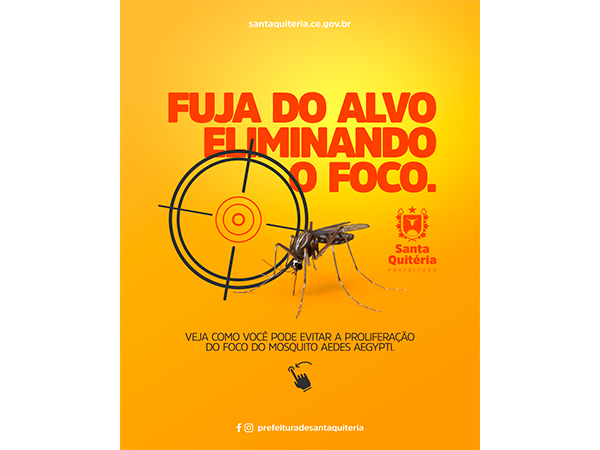
\includegraphics[width=2.84494in,height=2.84494in]{imgSAEB_7_POR/media/image6.png}

\begin{myquote}

Desgostoso com a existência medíocre na sua pequena cidade natal, 
um belo dia, aí pelos seus vinte e dois anos, aceitara o convite de um
engenheiro inglês que, por aquelas bandas, andava a explorar
terras e terrenos diamantíferos. Todos julgavam que o ``seu'' mister 
andasse fazendo isso; a verdade, porém, é que o sábio inglês fazia estudos
desinteressados. Fazia puras e platônicas pesquisas geológicas e mineralógicas.
O diamante não era o fim dos seus trabalhos; mas o povo, que teimava em ver,
pelos arredores da cidade, o ventre da terra cheio de diamantes, não podia 
supor que um inglês que levava a catar pedras, pela manhã e até à noite,
tomando notas e com uns instrumentos rebarbativos, não estivesse com tais 
gatimonhas a caçar diamantes. Não havia meio do mister convencer à simplória 
gente do lugar que ele não queria saber de diamantes. 

\end{myquote}

\fonte{Lima Barreto. Clara dos Anjos. 
Disponível em: http://www.dominiopublico.gov.br/download/texto/bn000048.pdf.
Acesso em: 25 mai. 2023.}

Levando em consideração o conjunto do parágrafo, a expressão que melhor 
sintetiza o respeito do povo para com o estrangeiro sonhador é

\begin{escolha}

    \item engenheiro inglês.

    \item ``seu'' mister.

    \item o sábio inglês. 

    \item um inglês que levava a catar pedras

\end{escolha}